\documentclass[12pt]{article}
\usepackage[utf8]{inputenc}
\usepackage[spanish]{babel}
\usepackage{siunitx}
% ---------------------------------------------------
%                       FONT 
% ---------------------------------------------------

\usepackage{cmbright}                               % Font
\documentclass{article}
\usepackage{siunitx}
\usepackage[hidelinks]{hyperref} % LINKS
\usepackage{caption}
\decimalpoint
\usepackage{mathtools}
\usepackage{amsmath}
\usepackage{amsthm}
\usepackage{amssymb}
\usepackage{graphicx}
\usepackage[margin=0.9in]{geometry}
\usepackage{fancyhdr}
\usepackage[inline]{enumitem}
\usepackage{float}
\usepackage{cancel}
\usepackage{bigints}
\usepackage[usenames]{color}
\usepackage{xcolor}
\usepackage{listingsutf8}
\usepackage{algorithm}
\usepackage{tocloft}
\usepackage[none]{hyphenat}
\usepackage{graphicx}
\usepackage{grffile}
\usepackage{tabularx}
\usepackage[nottoc,notlot,notlof]{tocbibind}
\usepackage{times}
\usepackage{color}
\usepackage{enumitem}
\usepackage{amsfonts}
\definecolor{gray97}{gray}{.97}
\definecolor{gray75}{gray}{.75}
\definecolor{gray45}{gray}{.45}
\renewcommand{\cftsecleader}{\cftdotfill{\cftdotsep}}
\pagestyle{fancy}
\setlength{\headheight}{15pt} 
\lhead{Práctica 6: Pulsos por minuto con Fotopletismógrafo}
\rhead{\thepage}
\lfoot{ESCOM-IPN}
\renewcommand{\footrulewidth}{0.5pt}
\setlength{\parskip}{0.5em}
\newcommand{\ve}[1]{\overrightarrow{#1}}
\newcommand{\abs}[1]{\left\lvert #1 \right\lvert}
\date{ 01 de Junio 2018}
\title{Amplificador}
\author{Instrumentacion}
\usepackage[
  separate-uncertainty = true,
  multi-part-units = repeat
]{siunitx}

\definecolor{pblue}{rgb}{0.13,0.13,1}
\definecolor{pgreen}{rgb}{0,0.5,0}
\definecolor{pred}{rgb}{0.9,0,0}
\definecolor{pgrey}{rgb}{0.46,0.45,0.48}
\lstset{tabsize=1}
\usepackage{wrapfig}
\usepackage{multicol}
\usepackage{listings}
\lstset{ frame=Ltb,
framerule=0pt,
aboveskip=0.5cm,
framextopmargin=3pt,
framexbottommargin=3pt,
framexleftmargin=0.4cm,
framesep=0pt,
rulesep=.4pt,
backgroundcolor=\color{gray97},
rulesepcolor=\color{black},
%
stringstyle=\ttfamily,
showstringspaces = false,
basicstyle=\small\ttfamily,
commentstyle=\color{gray45},
keywordstyle=\bfseries,
%
numbers=left,
numbersep=15pt,
numberstyle=\tiny,
numberfirstline = false,
breaklines=true,
}

% minimizar fragmentado de listados
\lstnewenvironment{listing}[1][]
{\lstset{#1}\pagebreak[0]}{\pagebreak[0]}

\lstdefinestyle{consola}
{basicstyle=\scriptsize\bf\ttfamily,
backgroundcolor=\color{gray75},
}

\lstdefinestyle{Java}
{language=Java,
}

    
%%%%%%%%%%%%%%%%%%%%%

\lstdefinestyle{customc}{
  belowcaptionskip=1\baselineskip,
  breaklines=true,
  frame=L,
  xleftmargin=\parindent,
  language=C,
  showstringspaces=false,
  basicstyle=\footnotesize\ttfamily,
  keywordstyle=\bfseries\color{green!40!black},
  commentstyle=\itshape\color{purple!40!black},
  identifierstyle=\color{blue},
  stringstyle=\color{orange},
}

\lstdefinestyle{customasm}{
  belowcaptionskip=1\baselineskip,
  frame=L,
  xleftmargin=\parindent,
  language=[x86masm]Assembler,
  basicstyle=\footnotesize\ttfamily,
  commentstyle=\itshape\color{purple!40!black},
}

\lstset{escapechar=@,style=customc}

% Ayuda para el formato de las tablas
\usepackage{array}
% Se declara un nuevo tipo de columna para alinear de manera:
% -Horizontal
\newcolumntype{P}[1]{>{\centering\arraybackslash}p{#1}}
% -Vertical
\newcolumntype{M}[1]{>{\centering\arraybackslash}m{#1}}

% Indica la separacion entre las columnas de una tabla
\setlength{\tabcolsep}{10pt} % Default value: 6pt
% Indica el padding inferior y superior de las celdas de una tabla
\renewcommand{\arraystretch}{1.8} % Default value: 1
% minimizar fragmentado de listados
\lstnewenvironment{listing}[1][]
{\lstset{#1}\pagebreak[0]}{\pagebreak[0]}

\lstdefinestyle{consola}
{basicstyle=\scriptsize\bf\ttfamily,
backgroundcolor=\color{gray75},
}

\lstdefinestyle{C}
{language=C,
}
 \lstset{style=CompilandoStyle}                                  %Use this style

    \usepackage{minted} % Paquete que permite citar codigo
    \usemintedstyle{borland} % Aqui se define el colorscheme para minted
    \setminted{
        fontsize = \scriptsize, % Ajusta el codigo a la hoja
        baselinestretch = 1,
        linenos, % set numbers
        breaklines=true, % Hace un salto de linea automatico en caso de que se llege al final de la line
        tabsize=3 
    }
%%%%%%%%%%%%%%%%%%%%%

\lstdefinestyle{customc}{
  belowcaptionskip=1\baselineskip,
  breaklines=true,
  frame=L,
  xleftmargin=\parindent,
  language=C,
  showstringspaces=false,
  basicstyle=\footnotesize\ttfamily,
  keywordstyle=\bfseries\color{green!40!black},
  commentstyle=\itshape\color{purple!40!black},
  identifierstyle=\color{blue},
  stringstyle=\color{orange},
}

\lstdefinestyle{customasm}{
  belowcaptionskip=1\baselineskip,
  frame=L,
  xleftmargin=\parindent,
  language=[x86masm]Assembler,
  basicstyle=\footnotesize\ttfamily,
  commentstyle=\itshape\color{purple!40!black},
}

\lstset{escapechar=@,style=customc}

    % =====  CODE EDITOR =========
    \lstdefinestyle{CompilandoStyle} {                              %This is Code Style
        backgroundcolor=\color{BlueGrey800MD},                      %Background Color  
        basicstyle=\tiny\color{white},                              %Font color
        commentstyle=\color{BlueGrey100MD},                         %Comment color
        stringstyle=\color{TealMD},                                 %String color
        keywordstyle=\color{Green100MD},                            %keywords color
        numberstyle=\tiny\color{TealMD},                            %Size of a number
        frame=shadowbox,                                            %Adds a frame around the code
        breakatwhitespace=true,                                     %Style                       
        breaklines=true,                                            %Style                   
        keepspaces=true,                                            %Style                   
        numbers=left,                                               %Style                   
        numbersep=10pt,                                             %Style 
        xleftmargin=\parindent,                                     %Style 
        tabsize=4                                                   %Style 
    }
 
    \lstset{style=CompilandoStyle}                                  %Use this style

    \usepackage{minted} % Paquete que permite citar codigo
    \usemintedstyle{borland} % Aqui se define el colorscheme para minted
    \setminted{
        fontsize = \scriptsize, % Ajusta el codigo a la hoja
        baselinestretch = 1,
        linenos, % set numbers
        breaklines=true, % Hace un salto de linea automatico en caso de que se llege al final de la line
        tabsize=3 
    }
    
\usepackage{longtable}
%Permite crear columnas en el documento
\usepackage{multicol}
\usepackage{color}
\usepackage{comment}
\newcommand{\tabitem}{~~\llap{\textbullet}~~}
\newcommand{\subtabitem}{~~~~\llap{\textbullet}~~}

\bibliographystyle{IEEEtran}
\begin{document}
        \begin{titlepage}
            \begin{center}
                
                % Upper part of the page. The '~' is needed because \\
                % only works if a paragraph has started.
                
                \noindent
                \begin{minipage}{0.5\textwidth}
                    \begin{flushleft} \large
                        \includegraphics[width=0.5\textwidth]{../ipn.png}
                    \end{flushleft}
                \end{minipage}%
                \begin{minipage}{0.55\textwidth}
                    \begin{flushright} \large
                        \includegraphics[width=0.4\textwidth]{../escom.png}
                    \end{flushright}
                \end{minipage}
                
                \textsc{\LARGE Instituto Politécnico Nacional}\\[0.5cm]
                
                \textsc{\Large Escuela Superior de Cómputo}\\[1cm]
                
                % Title
                
                { \huge Práctica 6: Pulsos por minuto con Fotopletismógrafo \\[1cm] }
                
                { \Large Unidad de aprendizaje: Instrumentación} \\[1cm]
                
                { \Large Grupo: 3CM4 } \\[1cm]
                
                \noindent
                \begin{minipage}{0.5\textwidth}
                    \begin{flushleft} \large
                        \emph{Integrantes:}\\
                        
                        \begin{tabular}{ll}
                        Aguilar Herrera Arianna Itzamina \\
                        Nicolás Sayago Abigail\\
                        Ramos Diaz Enrique \\
                    \end{tabular}
                    \end{flushleft}
                \end{minipage}%
                \begin{minipage}{0.5\textwidth}
                    \begin{flushright} \large
                        \emph{Profesor(a):} \\
                        Tellez Barrera Juan Carlos  \\
                    \end{flushright}
                \end{minipage}
                
                \vfill
                
                % Bottom of the page
                {\large Fecha de entrega: 17 de noviembre de 2018}
            \end{center}
        \end{titlepage}
    
    \tableofcontents
    
    % /////////////////////////////////////////////////////////////////////
    %                           OBJETIVOS
    % ////////////////////////////////////////////////////////////////////
    \section{Objetivo}
        \begin{itemize}
            \item[\checkmark] Aprender el uso y características del sensor de reflexión infrarrojo TCRT5000L
             \item[\checkmark] Graficar los pulsos del corazón con ayuda de un instrumento, el fotopletismógrafo. 
             \item[\checkmark] Programar una aplicación en Arduino para interpretar las señales de salida de un fotopletismografo.
             \item[\checkmark] Enviar las mediciones de los pulsos por minuto a un dispositivo móvil, por medio de conexión Bluetooth.
        \end{itemize}
    
    
        % /////////////////////////////////////////////////////////////////////
    %                           EQUIPO
    % ////////////////////////////////////////////////////////////////////
    \section{Listado de materiales}
        
        \begin{multicols}{2}
        
            \textbf{Resistores:}
            \begin{itemize}
                \item 1 de 150 $\Omega$
                \item 3 de 1 $k\Omega$
                \item 2 de 10 $k\Omega$
                \item 2 de 220 $k\Omega$
                \item 3 de 330 $k\Omega$
            \end{itemize}
            
            \textbf{Preset ó Potenciometro:}
            \begin{itemize}
                \item 1 de 10 $k\Omega$
            \end{itemize}
            
            \textbf{Capacitores:}
            \begin{itemize}
                \item 5 de $0.47$ microF o $470$ nanoF
                \item 1 de 100 $nF$
            \end{itemize}

      \columnbreak
    
          \textbf{Semiconductores:}
            \begin{itemize}
                \item 1 Sensor de reflexión infrarrojo TCRT5000L
                \item 1 Diodo LED
            \end{itemize}

        \textbf{Circuitos integrados:}
            \begin{itemize}
                \item 1 LM741 OPAMP  (alimentación $\pm12V$)
                \item Arduino Mega o Uno
                \item Módulo Bluetooth HC-05
            \end{itemize}   
            
        \textbf{Opcionales:}
            \begin{itemize}
                \item 1 Transistor BC547
                \item 1 Resistor 1$K\Omega$
            \end{itemize}
      
      \end{multicols}
      
    \section{Listado de equipo}
      \begin{multicols}{2}
        \begin{itemize}
            \item 1 Fuente de alimentación.
            \columbreak
            \item 1 Osciloscopio y vultímetro digital
            \item Celular smartphone con Bluetooth superior a la versión 5 y Android superior a la versión 2.1
        \end{itemize}
        \end{multicols}
        
    
    % /////////////////////////////////////////////////////////////////////
    %                           INTRODUCCION
    % ////////////////////////////////////////////////////////////////////

    \section{Introducción}
        \subsection{Fotopletismógrafo}
        En teoría, el fotopletismógrafo es simple: mide la variación en la cantidad de luz que pasa a través de su dedo causada por la naturaleza pulsátil del flujo sanguíneo.
        
        \begin{figure}[h!]
                \centering
                \includegraphics[width=0.45\textwidth]{Practica5/Images/foto3.jpg}
            \end{figure}
            
        \begin{figure}[h!]
                \centering
                \includegraphics[width=\textwidth]{Practica5/Images/foto.PNG}
            \end{figure}
        
        
        Un fuente de luz infrarroja (LED) emite un haz sobre la piel para iluminar los vasos subcutáneos, estos reflejan parte de dicho haz dependiendo la cantidad de hematíes que contienen. La luz reflejada incide en un fotosensor (usualmente de cadmio-selenio) que la convierte en un voltaje equivalente. 
        
        Debido a que la piel absorbe más del  $90\%$ de la luz, el par diodo-fotosensor se acompaña de amplificadores y filtros que garantizan un voltaje adecuado. El ciclo cardíaco puede obtenerse midiendo el intervalo que existe entre cada pico de voltaje.
            
        La calidad de las mediciones realizadas utilizando esta técnica dependen de la ubicación del emisor y receptor de luz, las características de los tejidos de cada paciente, la calidad de los amplificadores y filtros, entre otros. No obstante, su uso es generalizado teniendo en cuenta su bajo costo y su carácter no invasivo
        
        La señal que se trata de observar consiste en variaciones muy pequeñas (cambios en la intensidad de la luz debidos al flujo de sangre hacia o desde el dedo), superpuestas a una señal constante grande (luz promedio que fluye a través del dedo).  
        
        Es solo la parte de la señal que varía con el tiempo la que se debe amplificar. Para deshacerse de la señal de CC se puede utilizar un filtro de pasa altas.   
        
        Para asegurarse de que la señal de interés (el fotopletismógrafo) no sea eliminada por el filtro, la frecuencia de corte del filtro debe ser inferior a aproximadamente 1 Hz (una frecuencia cardíaca típica).
        
        \subsection{Arduino}
        Arduino es una plataforma de creación de electrónica de código abierto, la cual está basada en hardware y software libre, flexible y fácil de utilizar para los creadores y desarrolladores. Esta plataforma permite crear diferentes tipos de microordenadores de una sola placa a los que la comunidad de creadores puede darles diferentes tipos de uso.
        
        El Arduino es una placa basada en un microcontrolador ATMEL. Los microcontroladores son circuitos integrados en los que se pueden grabar instrucciones, las cuales las escribes con el lenguaje de programación que puedes utilizar en el entorno Arduino IDE. Estas instrucciones permiten crear programas que interactúan con los circuitos de la placa.
        
        \begin{figure}[h!]
                \centering
                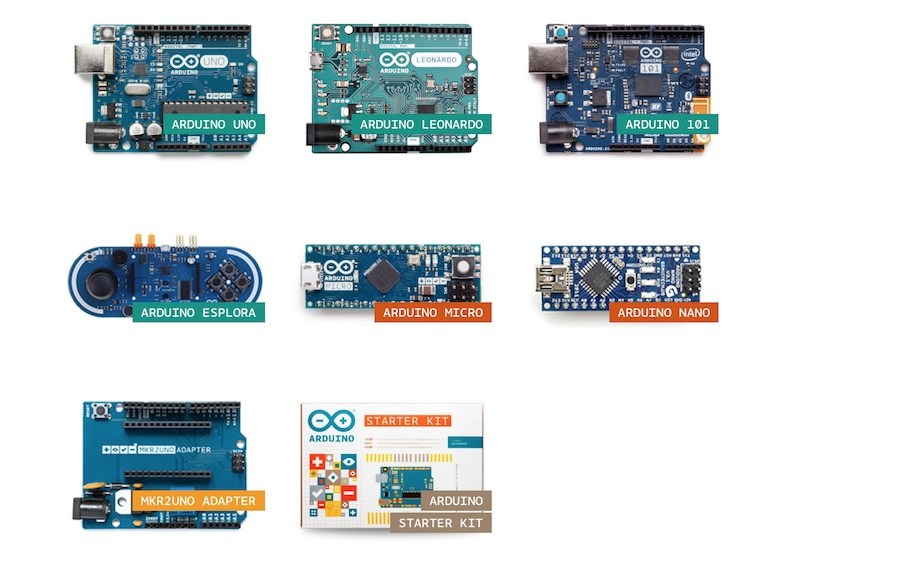
\includegraphics[width=0.7\textwidth]{Practica6/Images/arduino.jpeg}
            \end{figure}
            
        El microcontrolador de Arduino posee lo que se llama una interfaz de entrada, que es una conexión en la que podemos conectar en la placa diferentes tipos de periféricos. La información de estos periféricos que conectes se trasladará al microcontrolador, el cual se encargará de procesar los datos que le lleguen a través de ellos.
        
        El tipo de periféricos que puedas utilizar para enviar datos al microcontrolador depende en gran medida de qué uso le estés pensando dar. Pueden ser cámaras para obtener imágenes, teclados para introducir datos, o diferentes tipos de sensores.
        
        También cuenta con una interfaz de salida, que es la que se encarga de llevar la información que se ha procesado en el Arduino a otros periféricos. Estos periféricos pueden ser pantallas o altavoces en los que reproducir los datos procesados, pero también pueden ser otras placas o controladores.
        
        \subsection{Bluetooth}
        El Bluetooth Special Interest Group (SIG), una asociación comercial formada por líderes en telecomunicación, informática e industrias de red, está conduciendo el desarrollo de la tecnología inalámbrica Bluetooth y llevándola al mercado.

        La tecnología inalámbrica Bluetooth es una tecnología de ondas de radio de corto alcance (2.4 gigahertzios de frecuencia) cuyo objetivo es el simplificar las comunicaciones entre dispositivos informáticos, como ordenadores móviles, teléfonos móviles, otros dispositivos de mano y entre estos dispositivos e Internet. También pretende simplificar la sincronización de datos entre los dispositivos y otros ordenadores.
        
        Permite comunicaciones, incluso a través de obstáculos, a distancias de hasta unos 10 metros. Esto significa que, por ejemplo, puedes oír tus mp3 desde tu comedor, cocina, cuarto de baño, etc. También sirve para crear una conexión a Internet inalámbrica desde tu portátil usando tu teléfono móvil. Un caso aún más práctico es el poder sincronizar libretas de direcciones, calendarios etc en tu PDA, teléfono móvil, ordenador de sobremesa y portátil automáticamente y al mismo tiempo.
        
        \begin{figure}[h!]
                \centering
                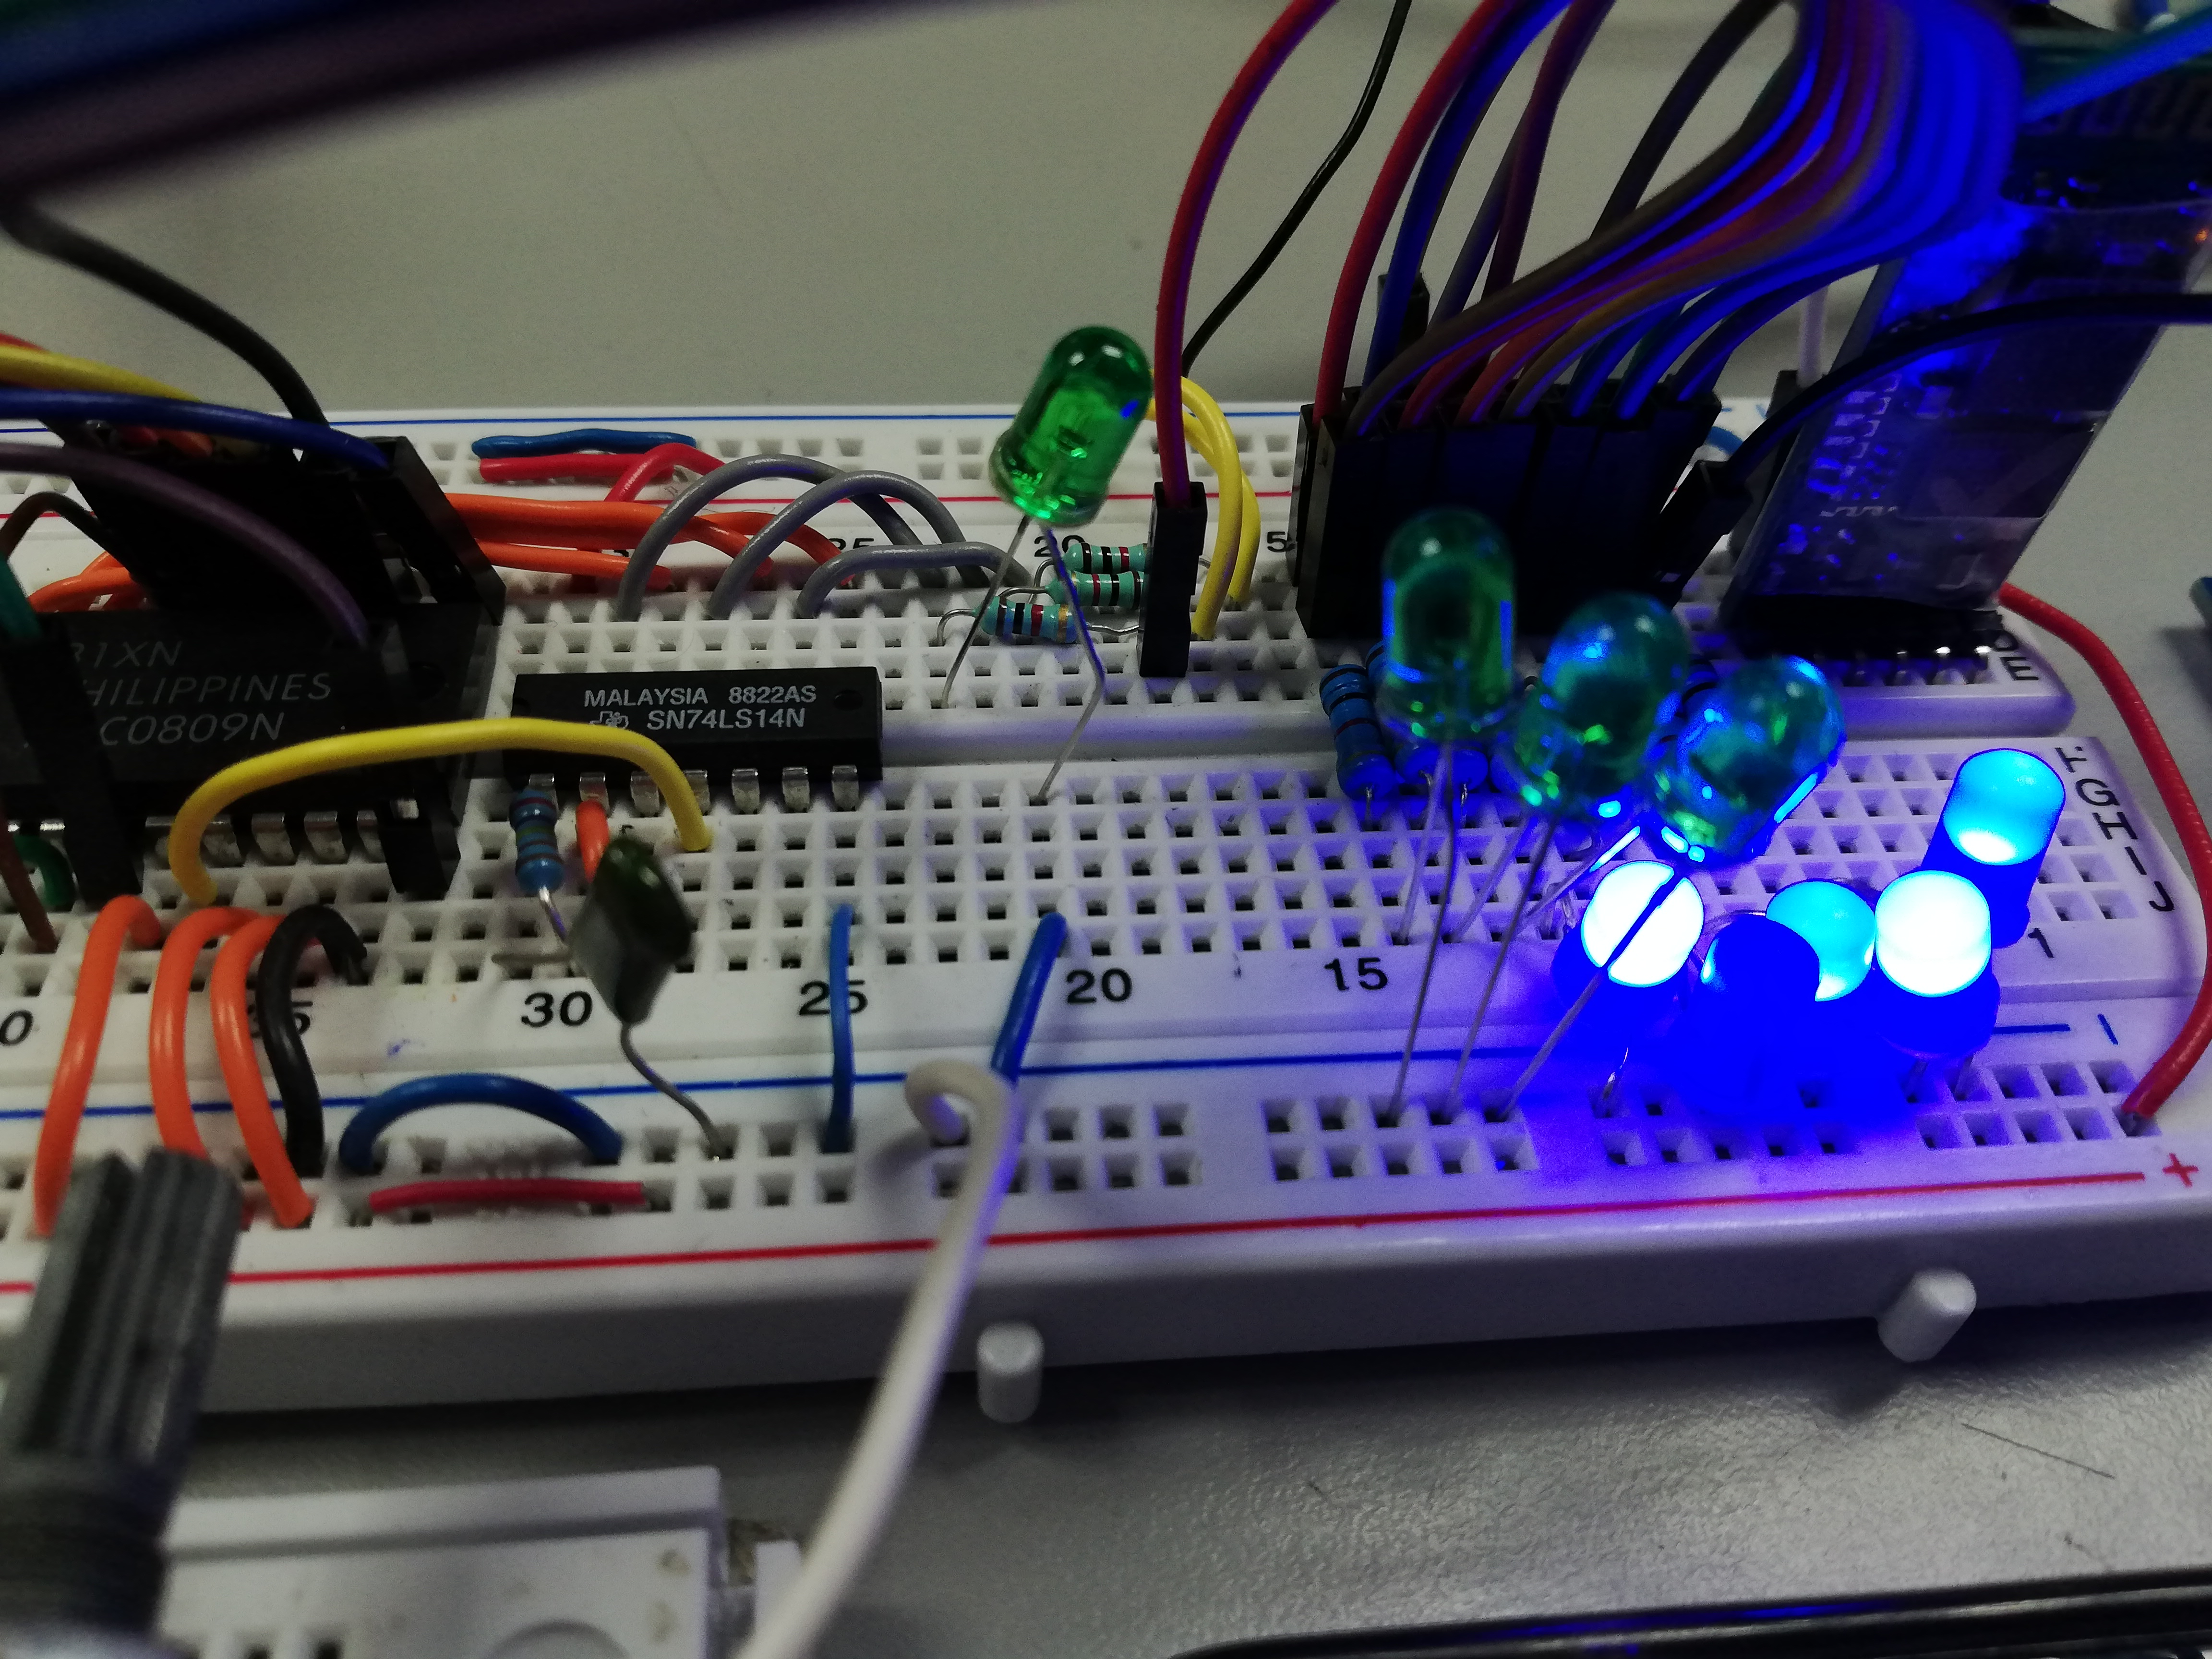
\includegraphics[width=0.6\textwidth]{Practica6/Images/bluetooth.jpg}
            \end{figure}
    % /////////////////////////////////////////////////////////////////////
    %                           DESARROLLO
    % ////////////////////////////////////////////////////////////////////
    \newpage
    \section{Desarrollo práctico}
    \subsection{Recordando la práctica 5}
    En la práctica anterior acondicionamos un sensor TCRT5000L para realizar un fotopletismografo, un circuito que mide las pulsaciones cardiacas de un individuo por medio de los cambios de luz que genera la sangre en los dedos de la mano.
    
    Ahora bien, en aquella práctica únicamente llegamos hasta la etapa de un comparador. En ésta práctica vamos a interpretar esta señal obtenida como el número de pulsos del corazón por minuto, por medio de una aplicación móvil y Arduino.
    
    Antes de entrar de lleno a la parte de Arduino, Bluetooth y Android, primero debemos realizar un ligero ajuste.
    
    \subsection{PE 1 - Transistor como interruptor}
    
    \begin{multicols}{2}
            \subsubsection{Esquema de conexión}

                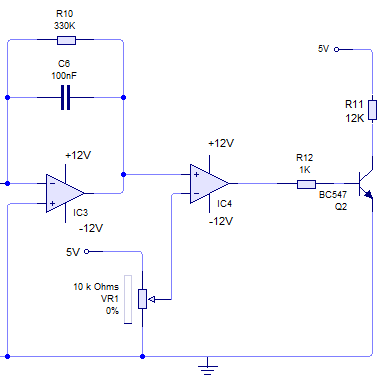
\includegraphics[width=0.5\textwidth]{Practica6/Images/ctransistor.png}

        \columnbreak
            \subsubsection{Circuito cableado}

                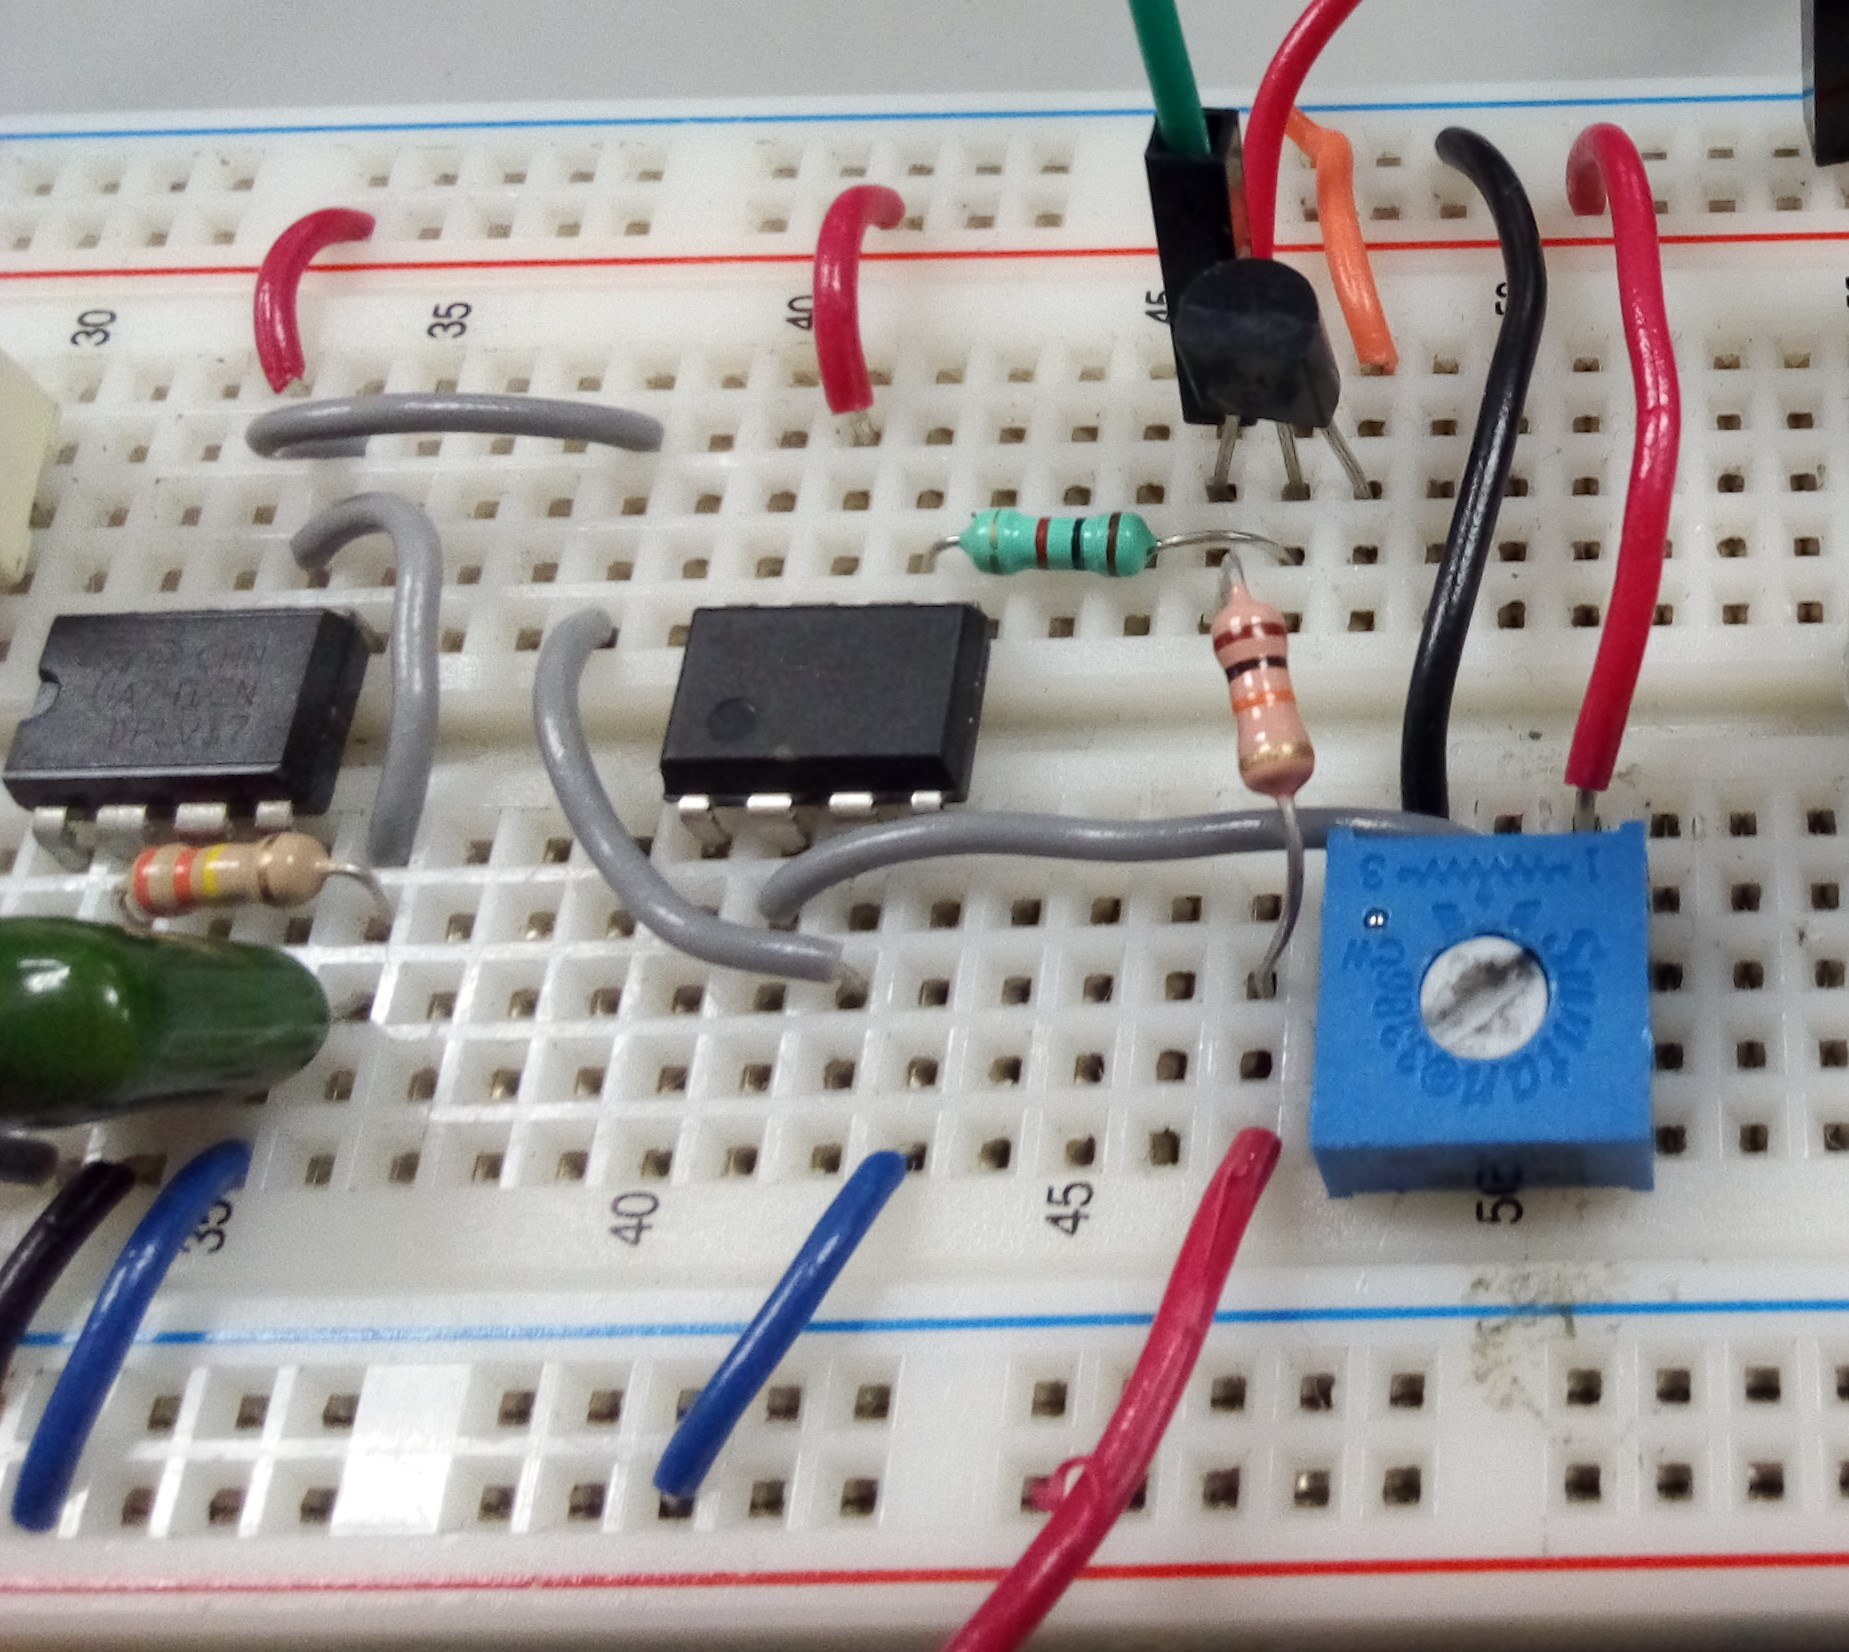
\includegraphics[width=0.5\textwidth]{Practica6/Photos/transistor.jpg}

            \end{multicols}
    
    \subsubsection{Funcionamiento}
    Tomando el circuito anterior, debemos de quitar el LED y su resistencia que encendía a cada pulso cardíaco, y en su lugar colocar un transistor BC547, que va a funcionar como interruptor que limita la salida del comparador de voltaje a 5V, entregándonos una señal cuadrada (quitamos el LED para no reducir la corriente que debe ir hacia el transistor). 
    
    Específicamente, cuando el sensor no detecta ningún cambio de luz, es decir, no existe pulso o no se ha colocado el dedo en él, la señal se mantendrá en 5 V constantes; cada vez que el sensor detecte un pulso, habrá un flanco de bajada hasta los 0 V, y cuando no se detecte nada, habrá un flanco de subida a 5 V nuevamente.
    
    \textbf{Parámetros de medición (Vpp)}
            \begin{multicols}{2}
                \begin{itemize}
                    \item[\checkmark] \textbf{Amplitud máxima: 5 V}
                
                    \item[\checkmark] \textbf{Base de tiempo: 1 s}
            \columnbreak
                    \item[\checkmark] \textbf{Volts por división: 5 V}
                    \item[\checkmark] \textbf{Acoplamiento: Corriente Continua}
                \end{itemize}
            \end{multicols}
    
    \textbf{Nota:} Nos interesa obtener una señal digital, que arroje valores lógicos de 1 (5V) y 0 (0V) para poder interpretarlas en Arduino. 
         
            \begin{figure}[h!]
                \centering
                \includegraphics[width=0.65\textwidth]{Practica6/Photos/senal.jpg}
            \end{figure}
    
    
    \newpage
    \subsection{PE 2 - Módulo Bluetooth HC-05 y placa Arduino}
    \subsubsection{Esquema de conexión}
    \begin{figure}[h!]
                \centering
                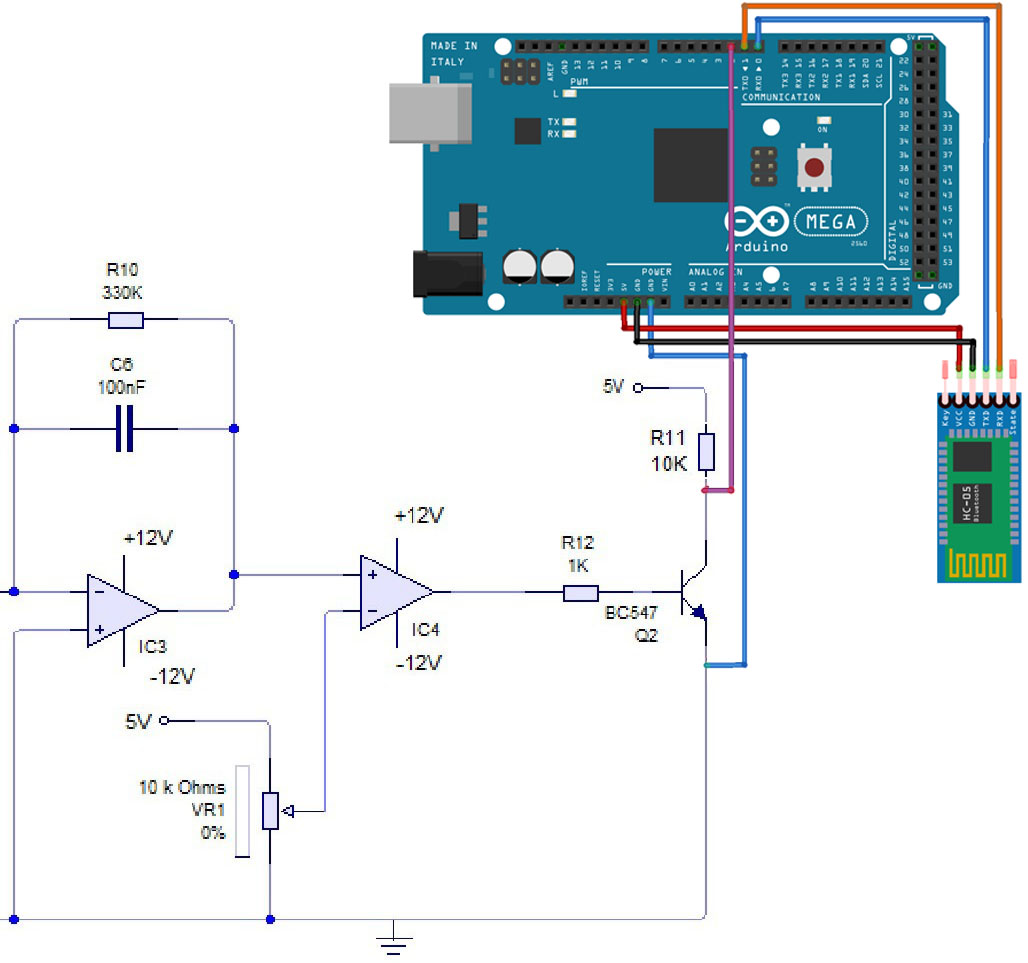
\includegraphics[width=0.65\textwidth]{Practica6/Images/arduinocirc.jpg}
    \end{figure}
    
    \subsubsection{Circuito cableado}
    \begin{figure}[h!]
                \centering
                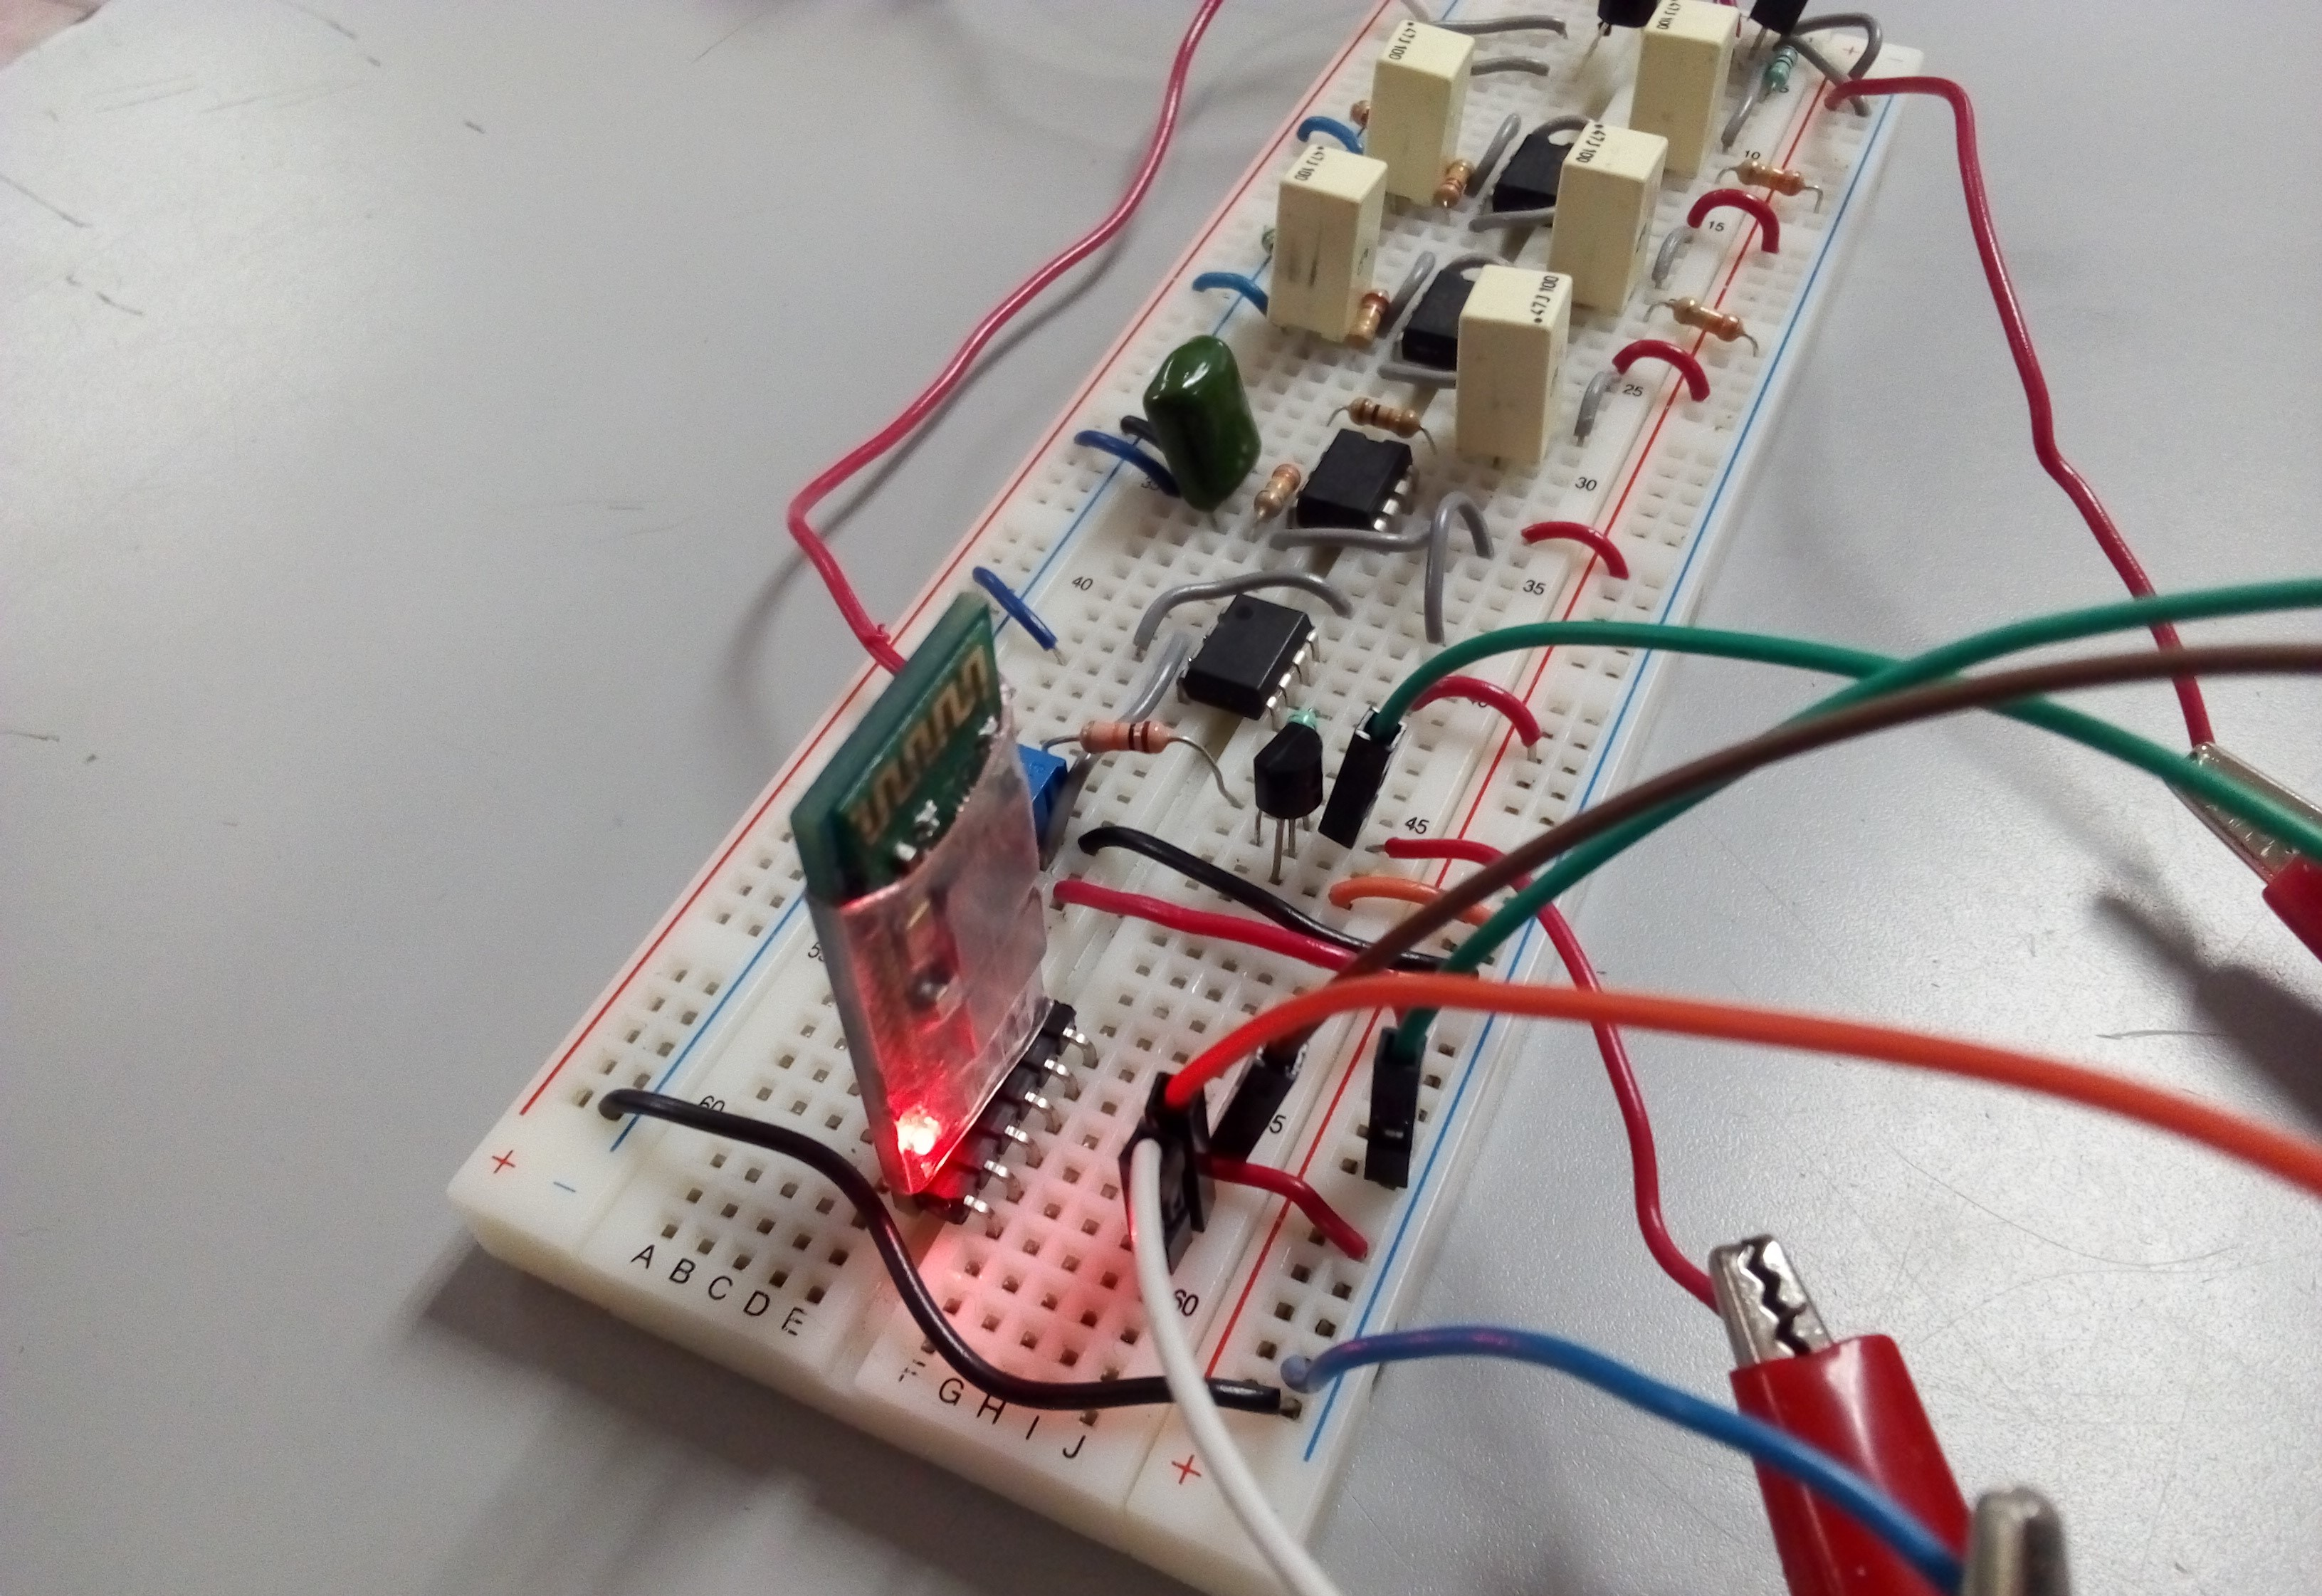
\includegraphics[width=0.65\textwidth]{Practica6/Photos/blue.jpg}
    \end{figure}
    
    \begin{figure}[h!]
                \centering
                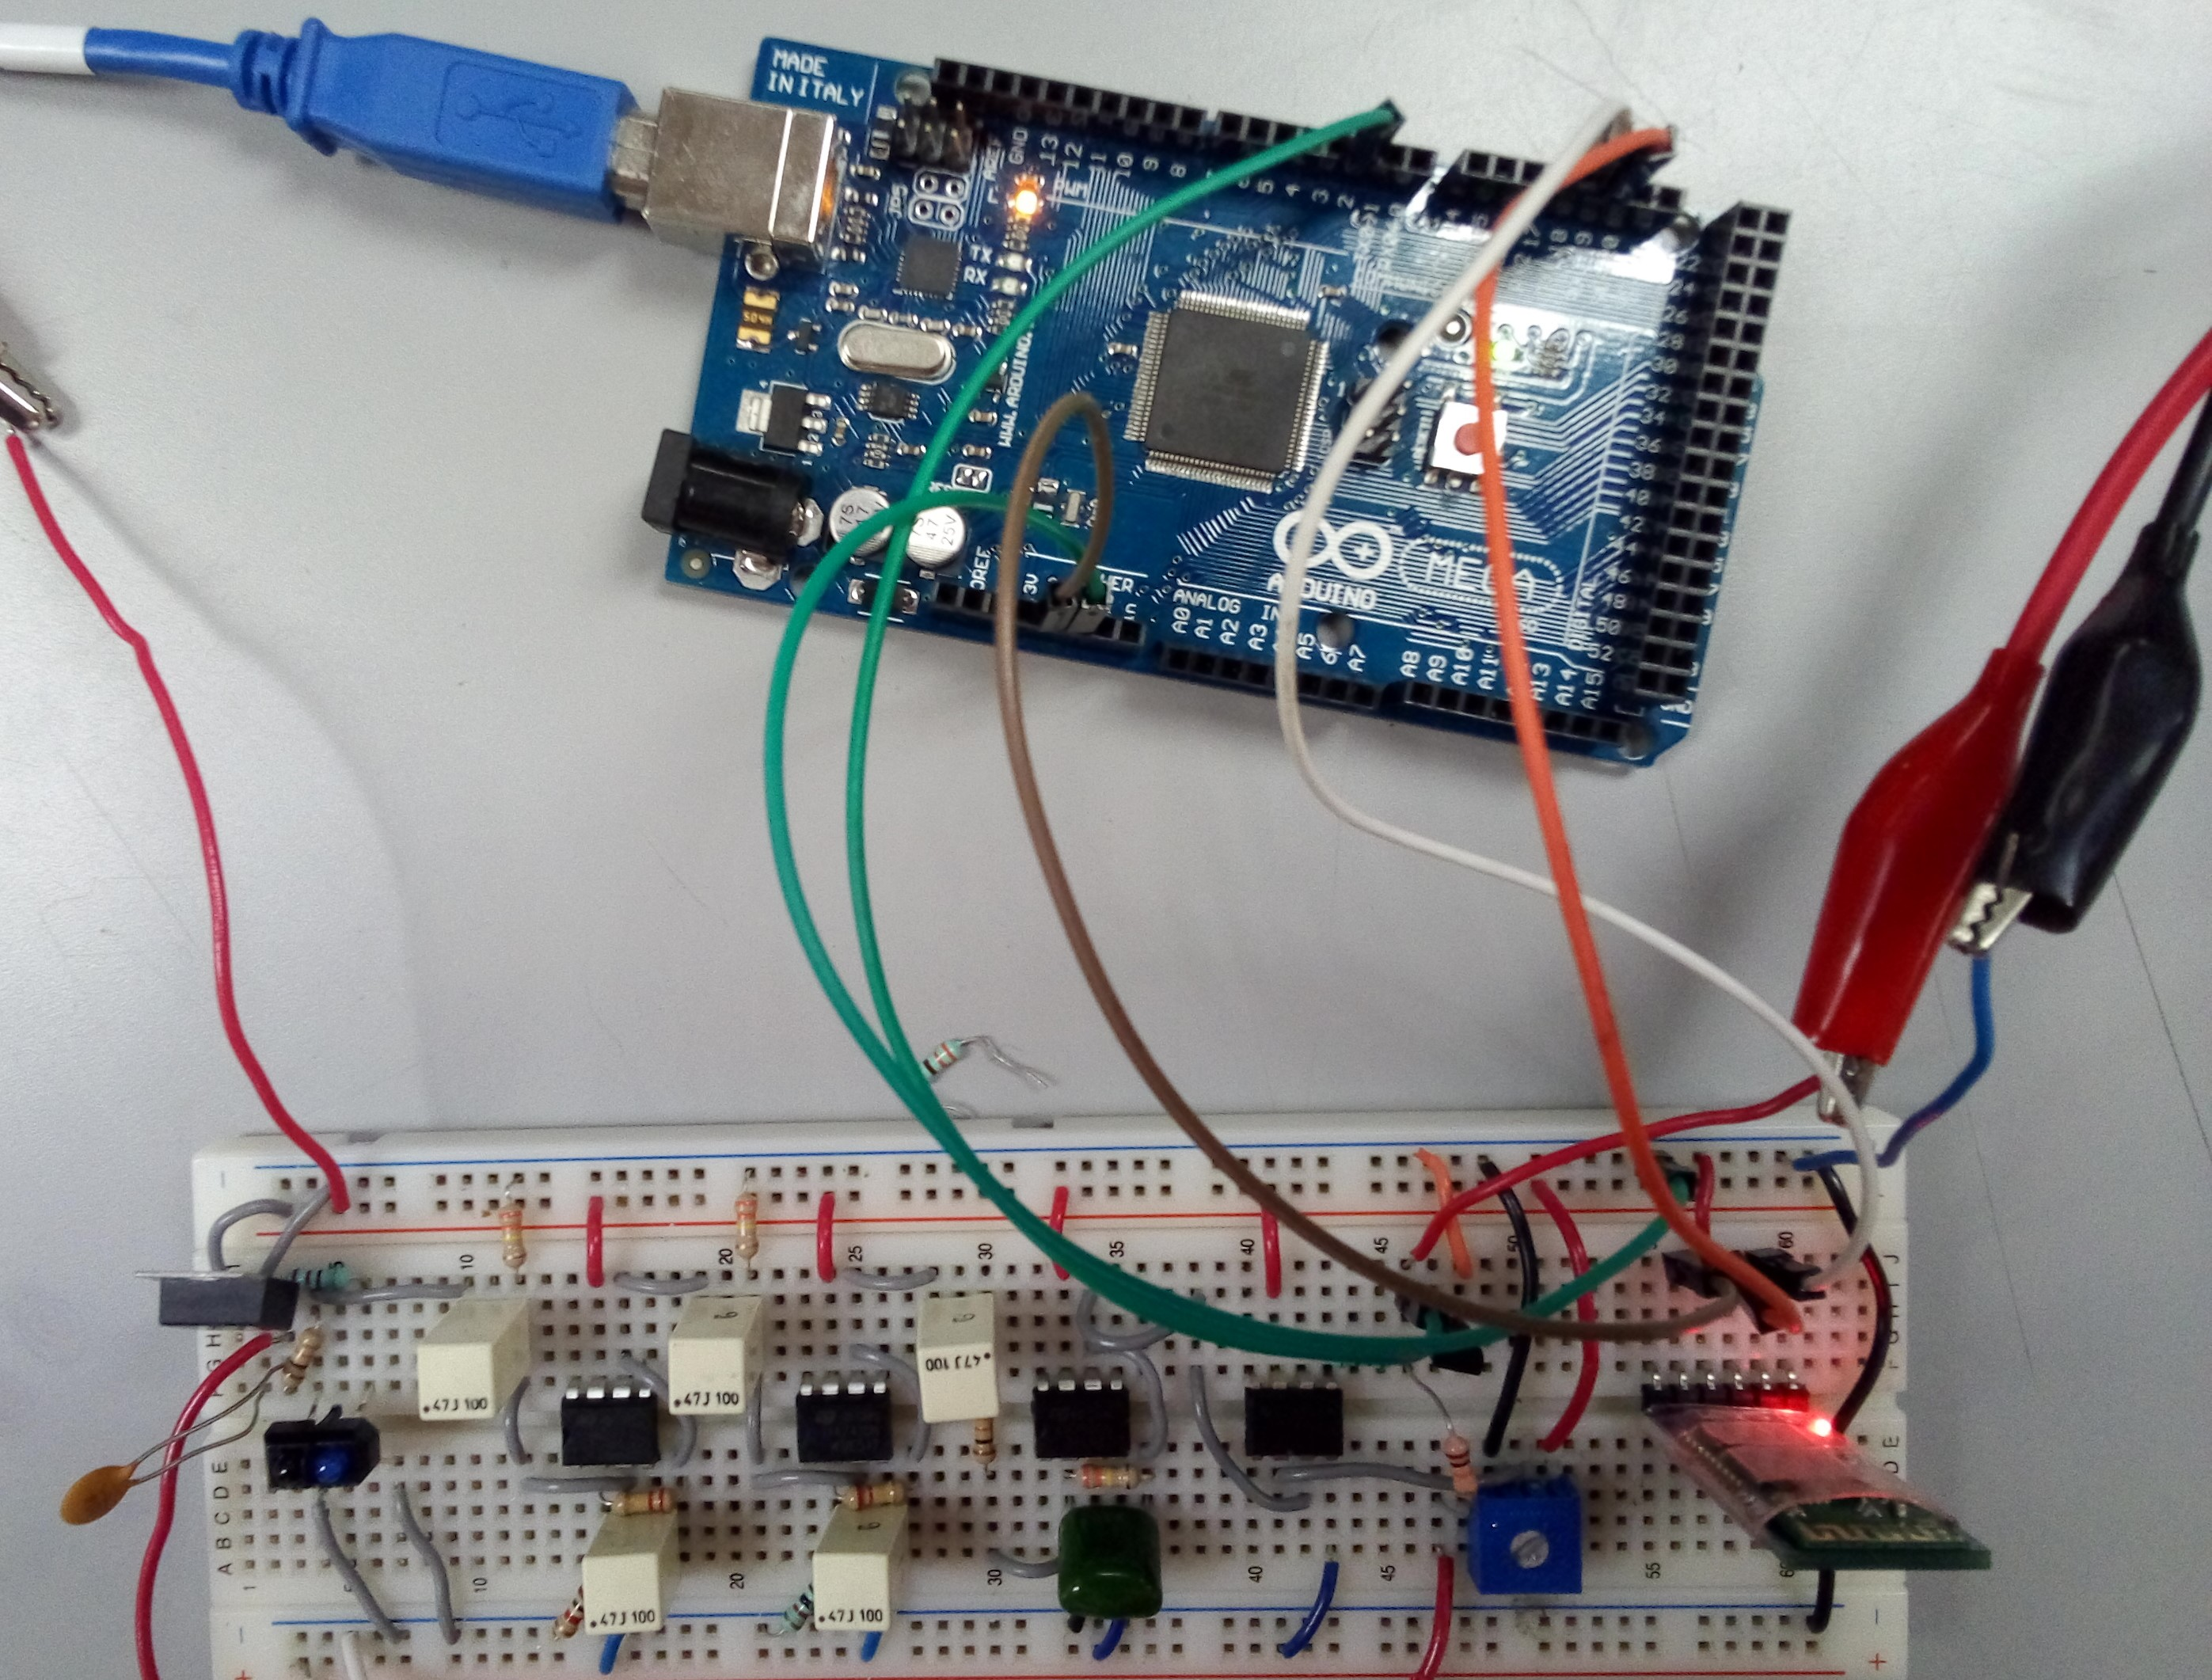
\includegraphics[width=0.65\textwidth]{Practica6/Photos/arduino.jpg}
    \end{figure}
    
    \subsubsection{Funcionamiento}
    La señal que sale de la pata colectora del transistor va ir directamente al pin 2 de la placa de Arduino.
    
    A su vez, enviamos el pin que entrega 5V al pin VCC del módulo Bluetooth HC-05, quien va a ser el encargado de transmitir la información codificada desde la placa de Arduino hacia nuestra aplicación Android en nuestro dispositivo móvil.
    
    Es de suma importancia cablear la salida del pin RX1 del Arduino hacia el pin TxD del HC-05, y de forma similar cablear la salida del pin TX1 del Arduino hacia el pin RxD del HC-05.
    
    Se colocan de forma cruzada, pues el pin RX1 de Arduino va a recibir datos por medio del pin TxD del HC-05 y viceversa, el pin RxD del HC-05 va a recibir datos por medio del pin TX1 de Arduino. Esta última línea de comunicación es la que nos interesa por ahora, pues la comunicación será unidireccional, de Arduino al módulo Bluetooth, y éste va a retransmitir los datos hacia el dispositivo móvil.
    
    No debemos olvidar colocar las tierras de ambos componentes en la tierra común del circuito fotopletismógrafo.
    
    \newpage
    \subsection{PE 3 - Programa en Arduino}
    \subsubsection{Código}
    \inputminted{Java}{Code/PULSE.c}
    
    \subsubsection{Explicación del código}
    Según la señal que esta continuamente entrando en el Arduino, debemos ser capaces de contar los cambios de flanco de éste entre 0 y 5 V, pues eso representa un pulso cardíaco obtenido en la lectura, en un periodo de tiempo de un minuto.
    
    Para ellos utilizamos interrupciones en Arduino, que son un mecanismo que permiten asociar una función a la ocurrencia de un determinado evento, en este caso, un pulso.
    
    Cuando ocurre el evento el procesador “sale” inmediatamente del flujo normal del programa y ejecuta la función de interrupción asociada ignorando por completo cualquier otra tarea (por esto se llama interrupción). Al finalizar la función de interrupción asociada, el procesador vuelve al flujo principal, en el mismo punto donde había sido interrumpido.
    
    En esta caso, nuestra función de interrupción esta definida como \textit{contar()}, y se ejecutará cada vez que hay un flanco de subida: \textit{\textbf{RISING}} en el pin 2, que es la señal que sale del transistor.
    
    
    
    Caqui leemos el tiempo anterior de que exista un flanco de subida, y leemos el tiempo posterior de este, que iremos guardando en variables globales. De éste modo, podemos calcular la duración del periodo total de cada flanco de subida, dividimos 60 segundos entre esta dato para obtener el número de pulsaciones.
    
    En el bloque \textit{setup()} inicializamos dos canales de comunicación seriales: \textbf{Serial} para visualizar los datos en la computadora, y \textbf{Serial1}, que corresponde al canal que maneja el Arduino para la comunicación Bluetooth, \textbf{este es el que nos interesa}.
    
    Y finalmente, definimos que el pin 2 es una entrada y que usaremos interrupciones con \textit{attachInterrupt()}.
    
    A su vez, en el bloque \textit{loop()}, tenemos una condición que posee un contador de tiempo y nos ayuda a saber cuándo ha pasado un segundo. Debajo de ésta, hay otra más que verifica que hayan transcurrido dos segundos en la ejecución del programa para imprimir los pulsos por minuto; debemos imprimir éste dato únicamente cuando sea menor a 120, pues el promedio de pulsos cardíacos por minuto en el ser humano esta entre 50 y 100 pulsos.
    \newpage
    \subsection{PE 4 - Aplicación Android desarrollada para móviles}
    \subsubsection{Código e interfaz gráfica}
    \begin{figure}[h!]
                \centering
                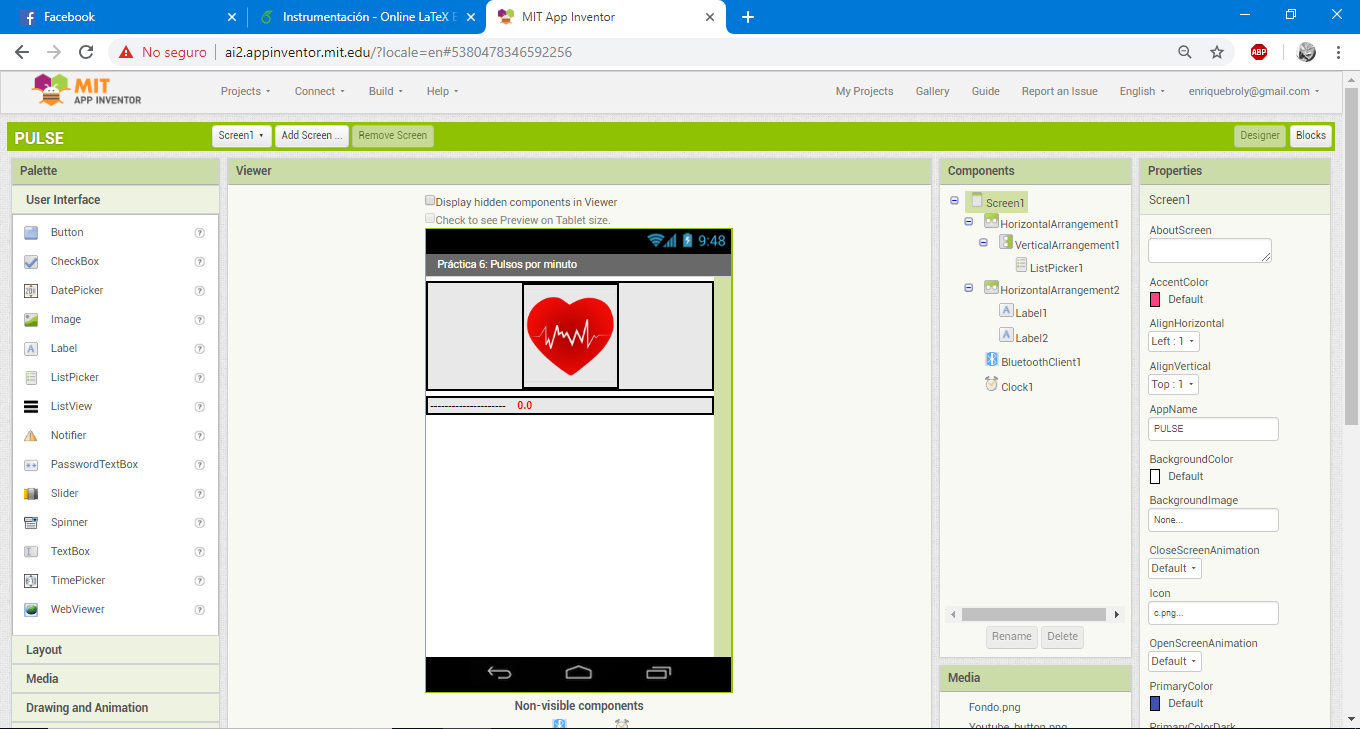
\includegraphics[width=\textwidth]{Practica6/Images/appinventor.PNG}
                 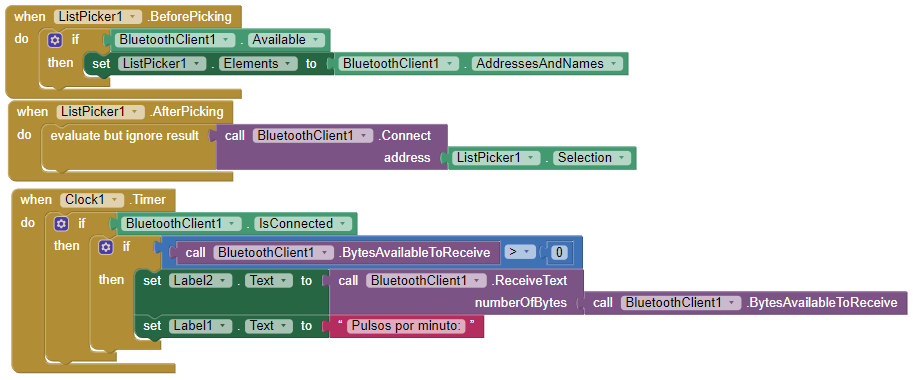
\includegraphics[width=\textwidth]{Practica6/Images/codeblocks.PNG}
    \end{figure}
    
    \subsubsection{Explicación del código}
    Para crear esta aplicación, utilizamos la página Web \textbf{MIT App Inventor}. 
    
    Primero creamos la interfaz gráfica, que consiste en un botón con una lista que contendrá todos los dispositivos Bluetooth emparejados que el dispositivo móvil posee (en donde se encuentra el icono del corazón), y un cuadro de texto en donde se mostrarán los pulsos por minuto.
    
    Además, contamos con dos elementos no visibles: un reloj para que nuestra aplicación este sincronizada con el temporizador del Arduino y los datos se muestren en tiempo real, \textbf{este debe ser inicializado en un valor de 1000 milisegundos, o un segundo}, y el cliente de conexión Bluetooth.
    
    Pasando a los bloques de código, primero le decimos a la aplicación que cada vez que se inicie, cargue todos los dispositivos Bluetooth emparejados al dispositivo móvil junto a su MAC.
    \begin{figure}[h!]
                \centering
             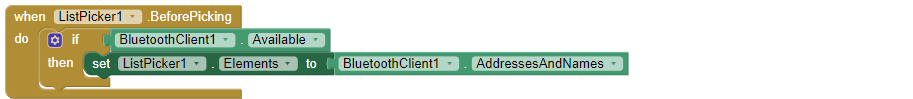
\includegraphics[width=\textwidth]{Practica6/Images/block1.PNG}
    \end{figure}
    
    Luego, decimos que al momento de seleccionar un dispositivo de la lista, la aplicación se conecte a él enviándole su dirección MAC por medio de la función\\
    \textit{call BluetoothClient1.Connectadress()}.
    
    \begin{figure}[h!]
                \centering
             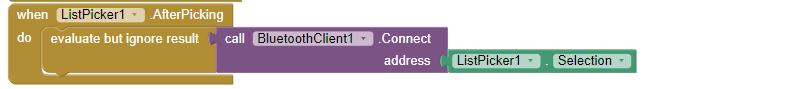
\includegraphics[width=\textwidth]{Practica6/Images/block2.PNG}
    \end{figure}
    
    Por último, cada vez que haya un pulso de reloj en la aplicación de un segundo, verificar que el cliente Bluetooth este conectado para así llamar a la función \textit{BytesAvailableToReceive()} y revisar que sí existan bytes que están siendo transmitidos. Si lo están, colocamos estos bytes en nuestros campos de texto con ayuda de la función \textit{ReceiveTextnumberOfBytes()}, para ir leeyendo la información desde el Arduino.
    
    \begin{figure}[h!]
                \centering
             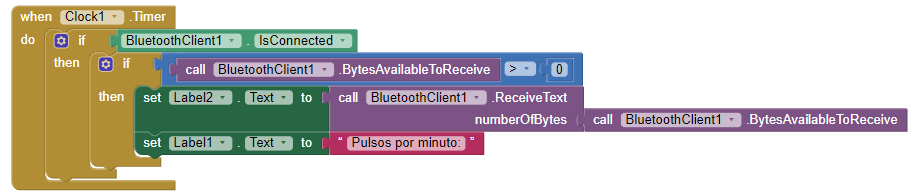
\includegraphics[width=\textwidth]{Practica6/Images/block3.PNG}
    \end{figure}
    
    Ésta información será la variable pulsos que enviamos por el canal \textbf{Serial1} en el código de Arduino.
    \newpage
    \subsubsection{Instalación}
    
    \begin{enumerate}
        \item Descargar e instalar el archivo ''PULSE.apk'' desde el móvil.
        \begin{figure}[h!]
                \centering
             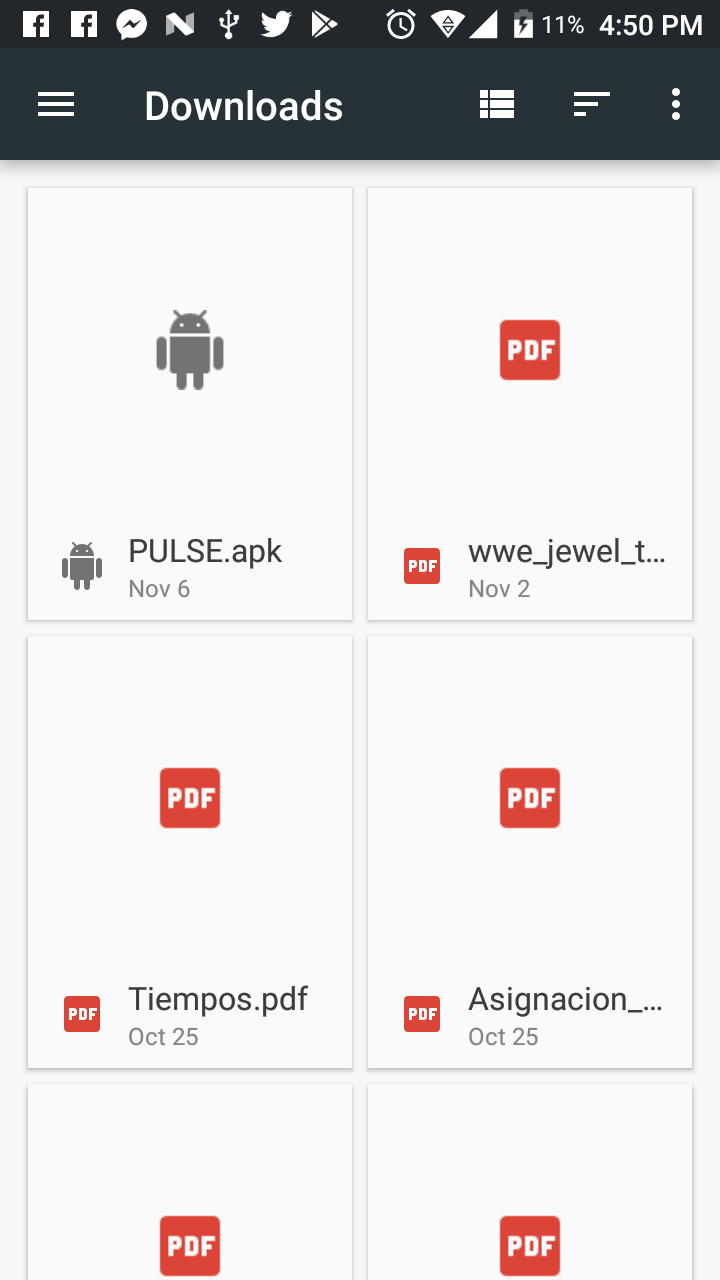
\includegraphics[scale=0.15]{Practica6/Images/ss1.png}
             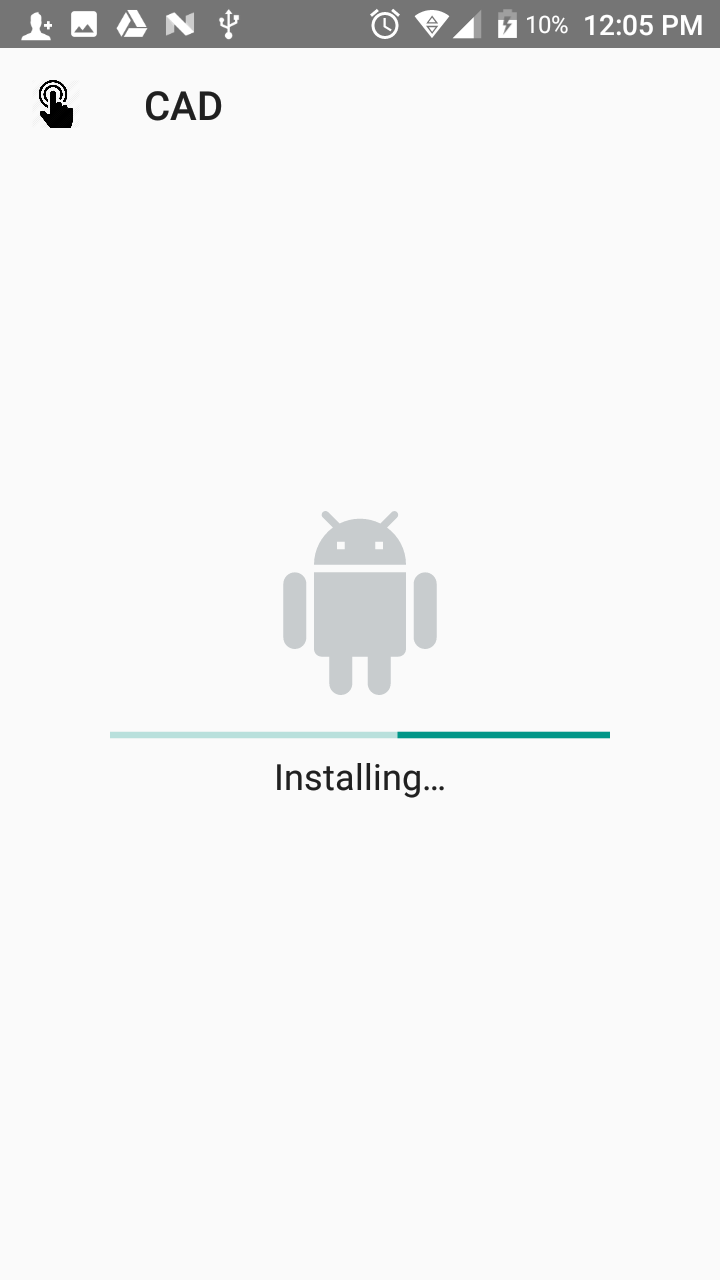
\includegraphics[scale=0.15]{Practica6/Images/ss2.png}
             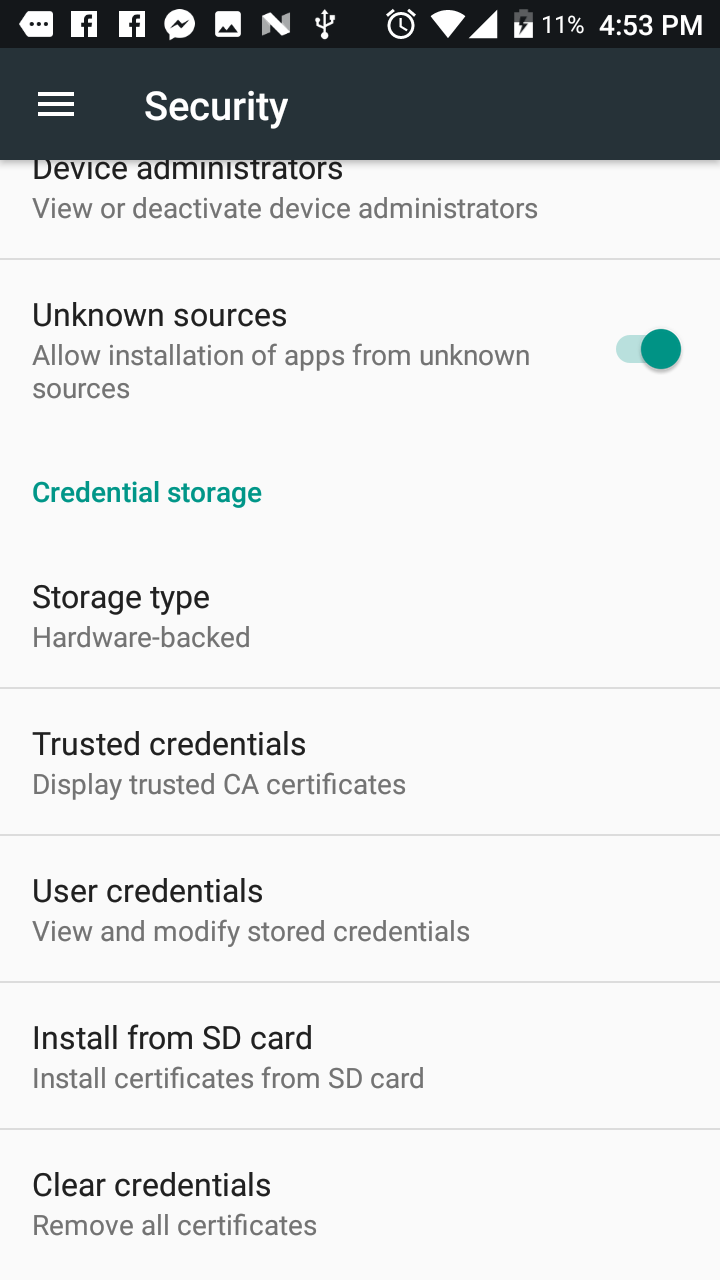
\includegraphics[scale=0.15]{Practica6/Images/ss3.png}
        \end{figure}
    
    \textbf{Importante}: Activar la opción de instalas aplicaciones de origen desconocido desde Ajustes.
        \item Activar el Bluetooth en el celular y emparejar el módulo HC-05 con el códgigo ''1234''.
        \item Entrar a la app.
        \item Pulsar el icono del corazón, aparecerá el listado de dispositivos Bluetooth, seleccionar el HC-05
        \item La app comenzará a desplegar las pulsaciones por segundo.
        
        \begin{figure}[h!]
                \centering
             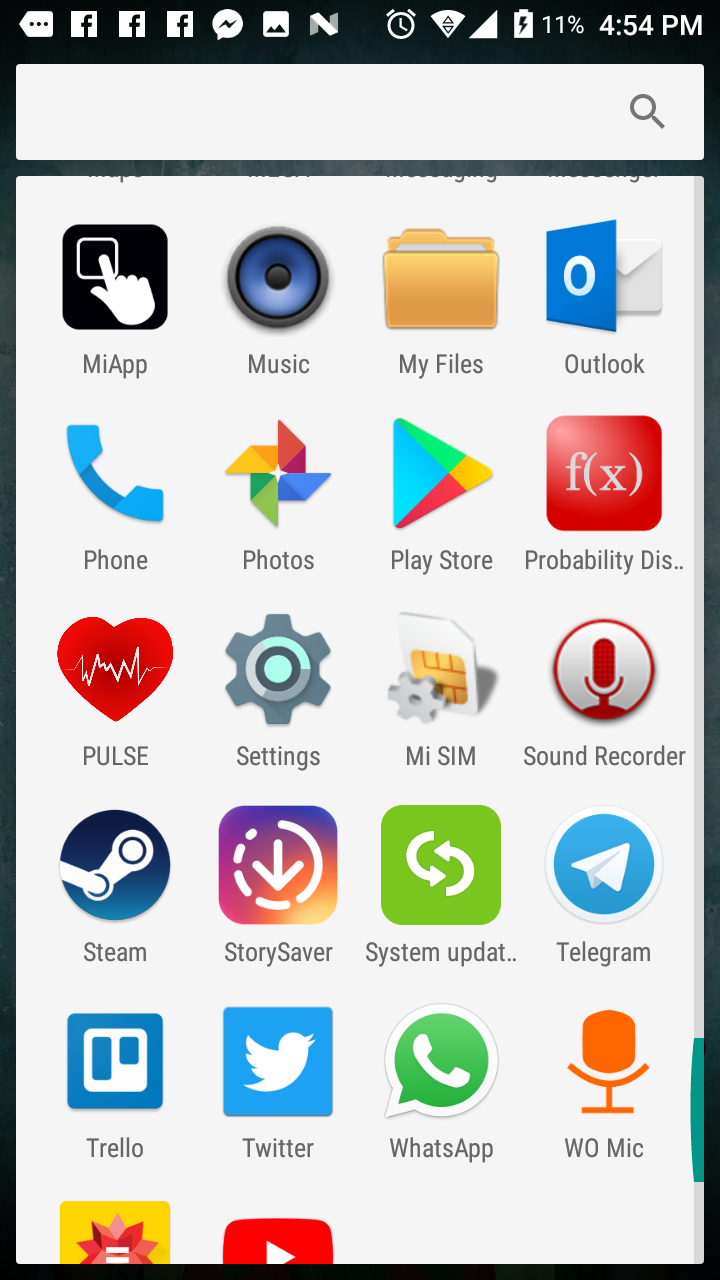
\includegraphics[scale=0.15]{Practica6/Images/ss4.png}
             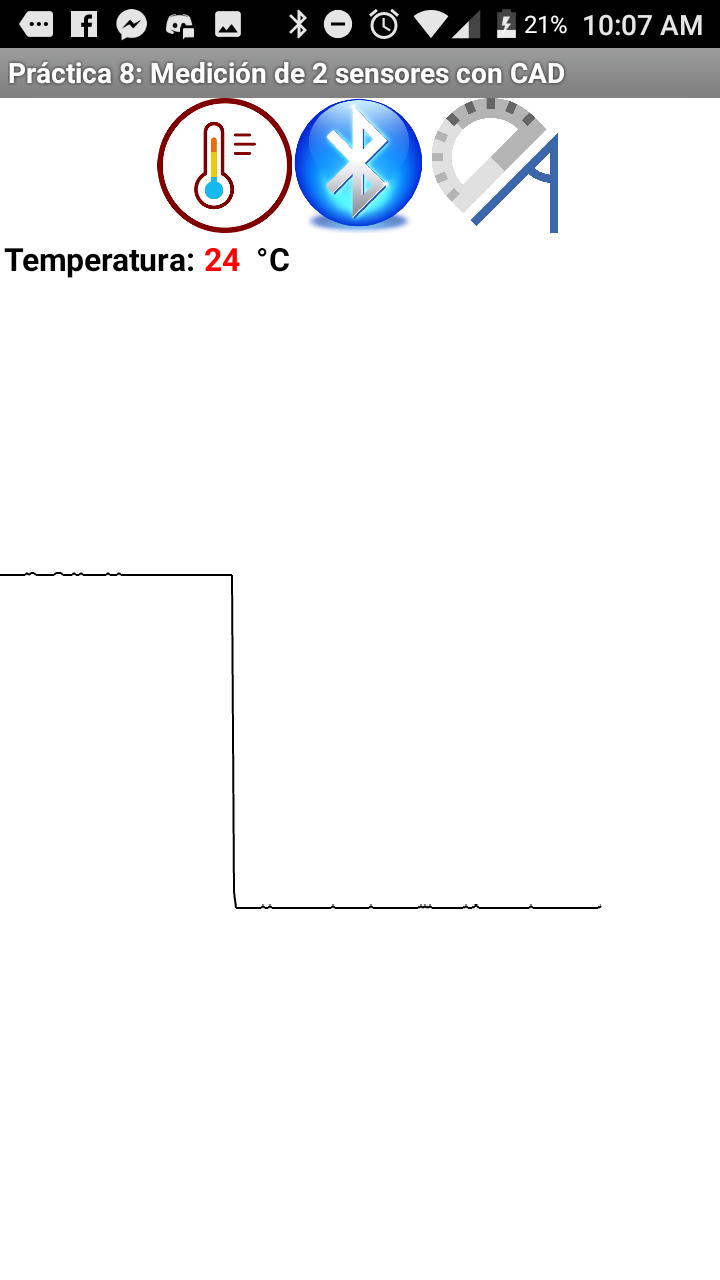
\includegraphics[scale=0.15]{Practica6/Images/ss5.png}
             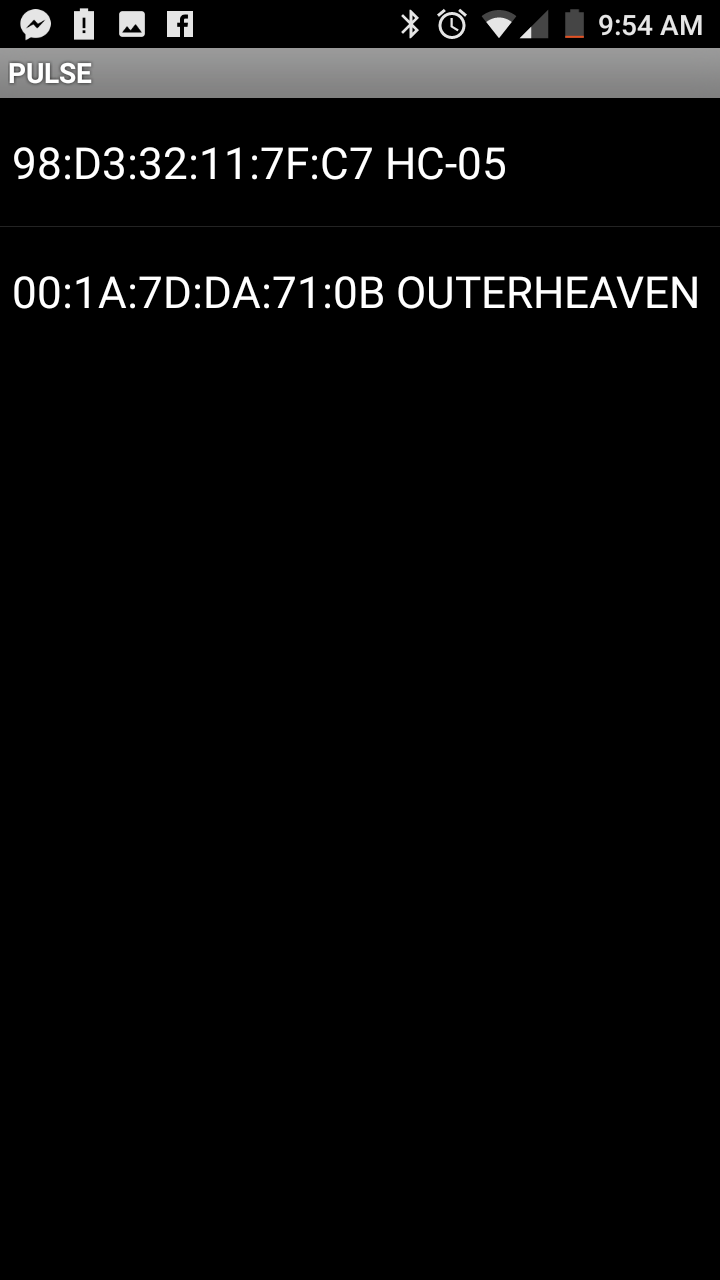
\includegraphics[scale=0.15]{Practica6/Images/ss6.png}
             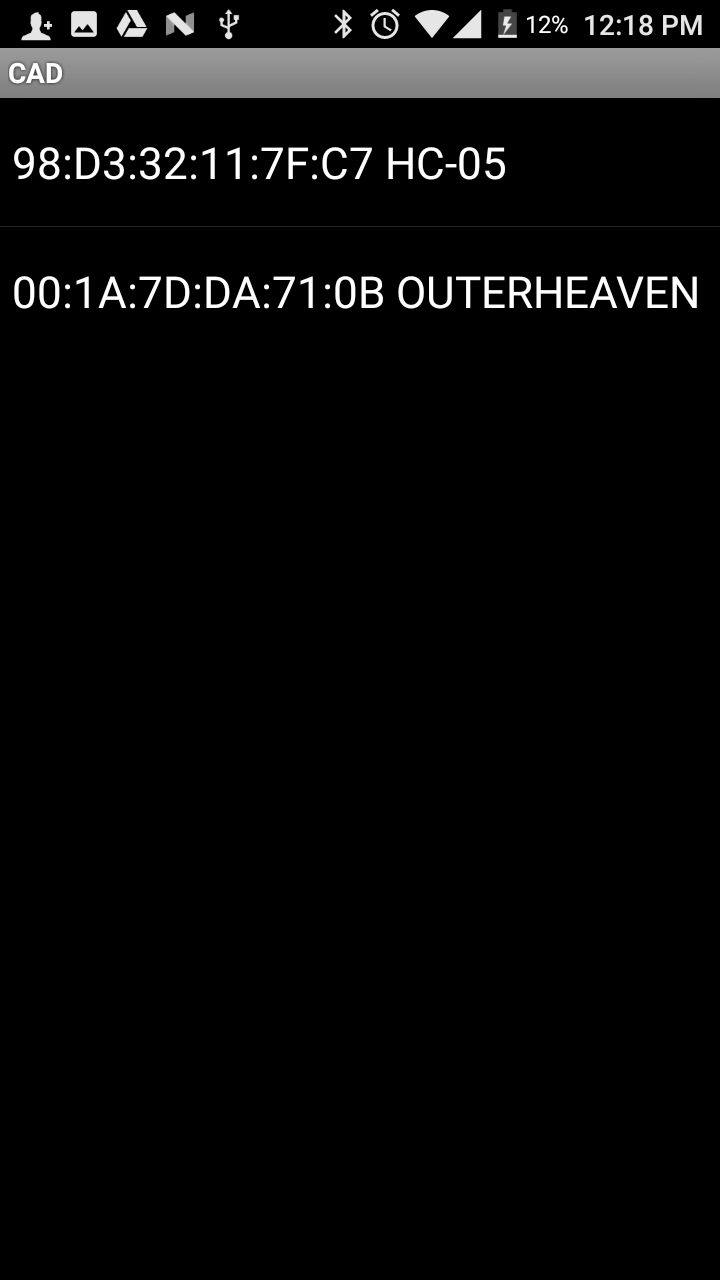
\includegraphics[scale=0.15]{Practica6/Images/ss7.png}
        \end{figure}
        
    \end{enumerate}
    
    \newpage
    \subsection{Funcionamiento completo}
    \begin{figure}[h!]
                \centering
             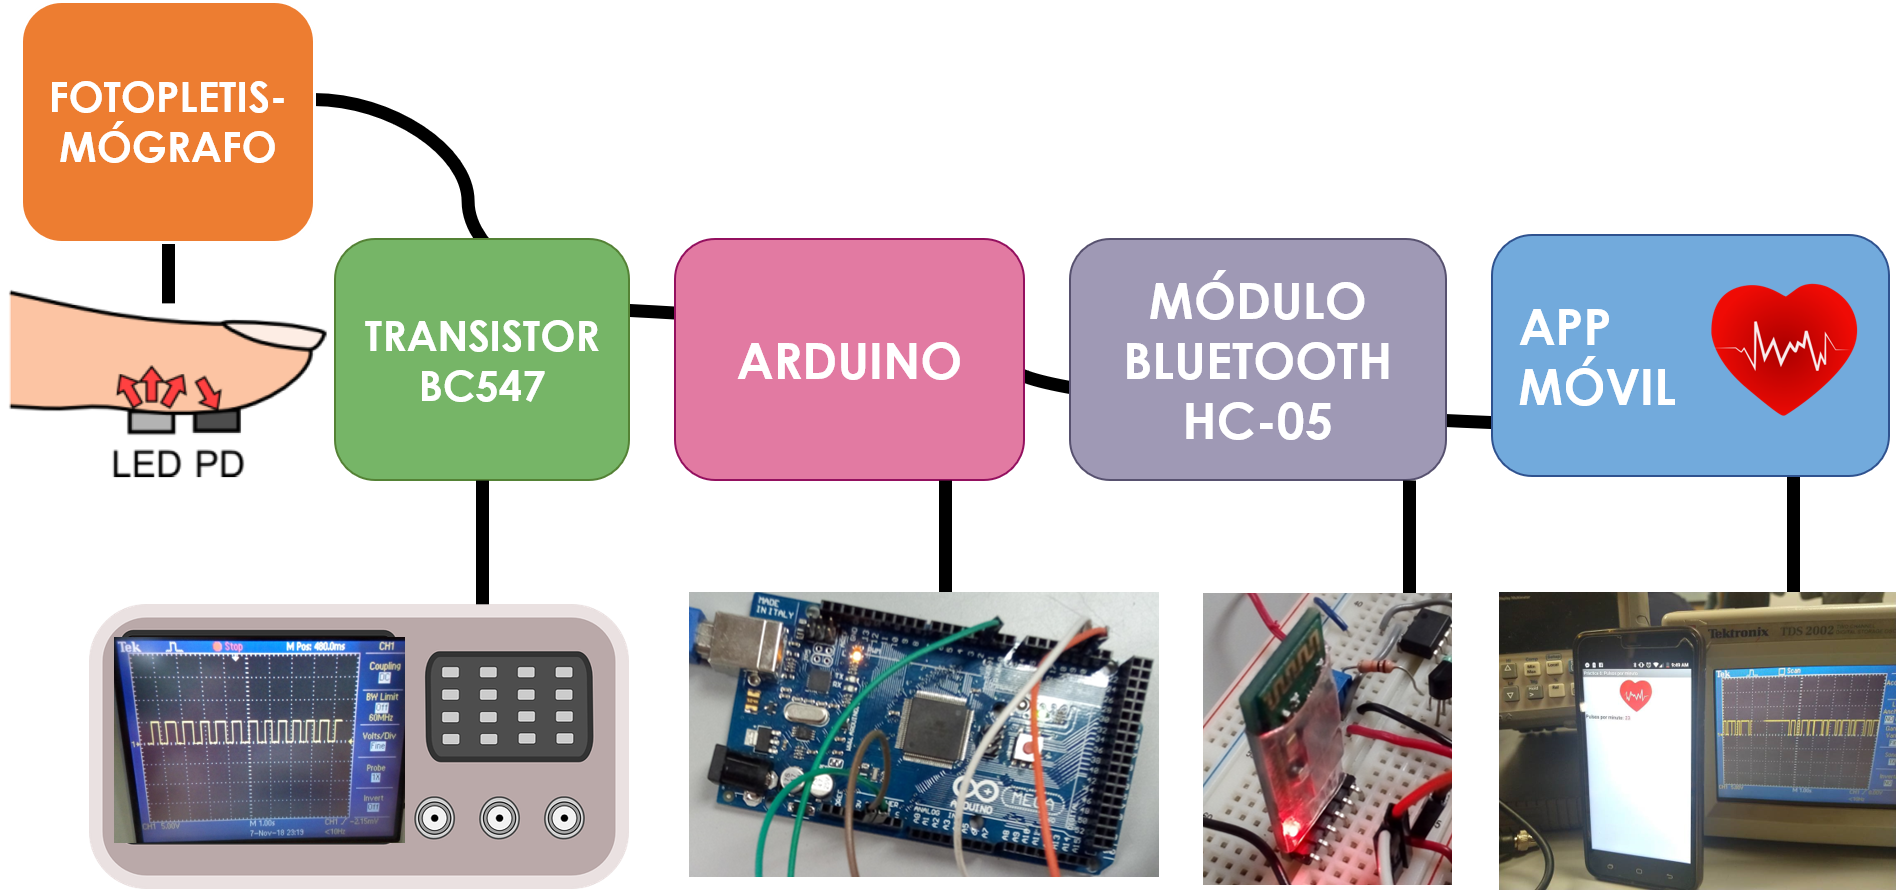
\includegraphics[width=\textwidth]{Practica6/Images/ETAPAS.png}
    \end{figure}
    
    \begin{itemize}
        \item Fotopletismografo: Entrega una señal que corresponde a los latidos cardíacos de una persona.
        \item Transistor BC547: Funciona como interruptor y limita la señal dentro de un rango de 0 a 5 V.
        \item Arduino: Calcula el periodo de cada pulso por minuto con ayuda de interrupciones y envía la cantidad de pulsos por minuto vía Bluetooth.
        \item Módulo Bluetooth HC-05: Retransmite la información recibida a un dispositivo móvil.
        \item App Móvil: Se conecta al HC-05 y despliega el número de pulsos por minuto en tiempo real.
    \end{itemize}
    \newpage
    \begin{figure}[h!]
                \centering
             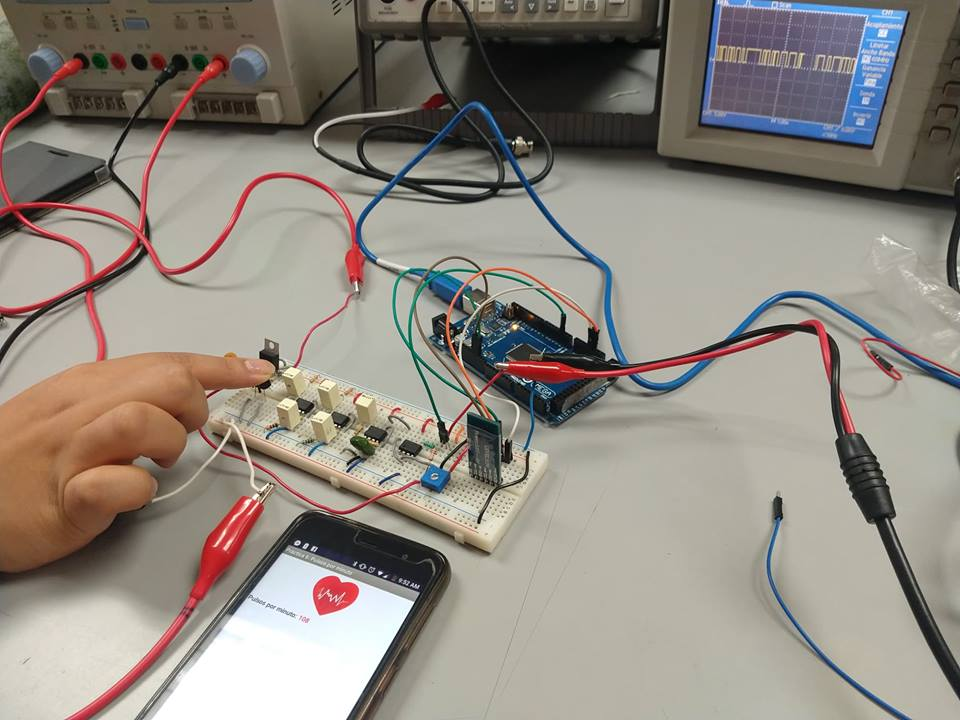
\includegraphics[width=0.8\textwidth]{Practica6/Photos/1.jpg}
             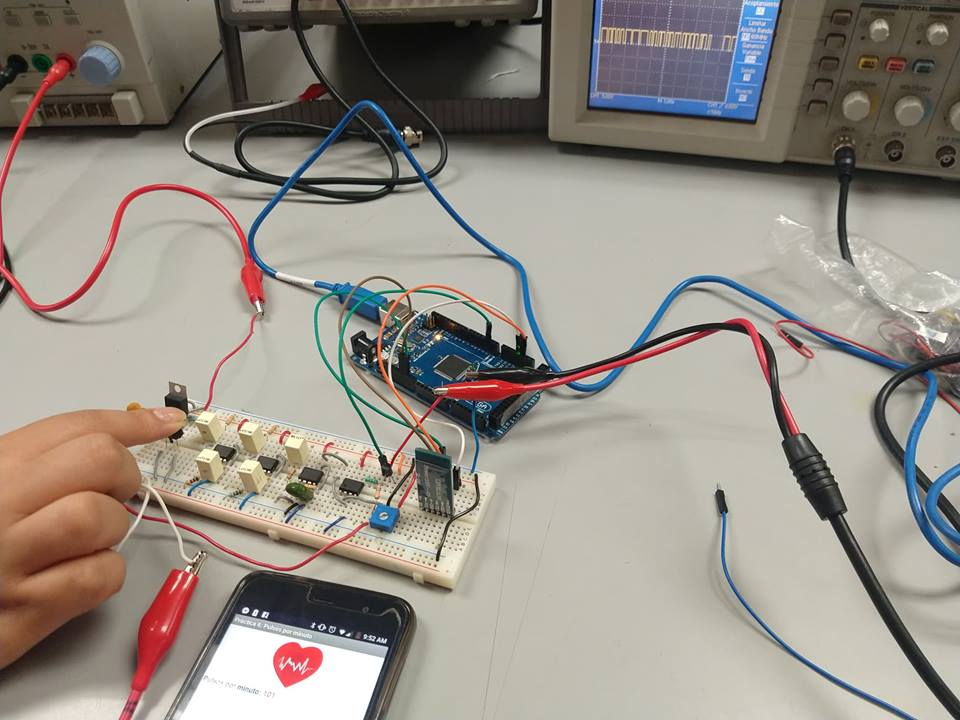
\includegraphics[width=0.8\textwidth]{Practica6/Photos/2.jpg}
    \end{figure}
    \newpage
    \begin{figure}[h!]
                \centering
             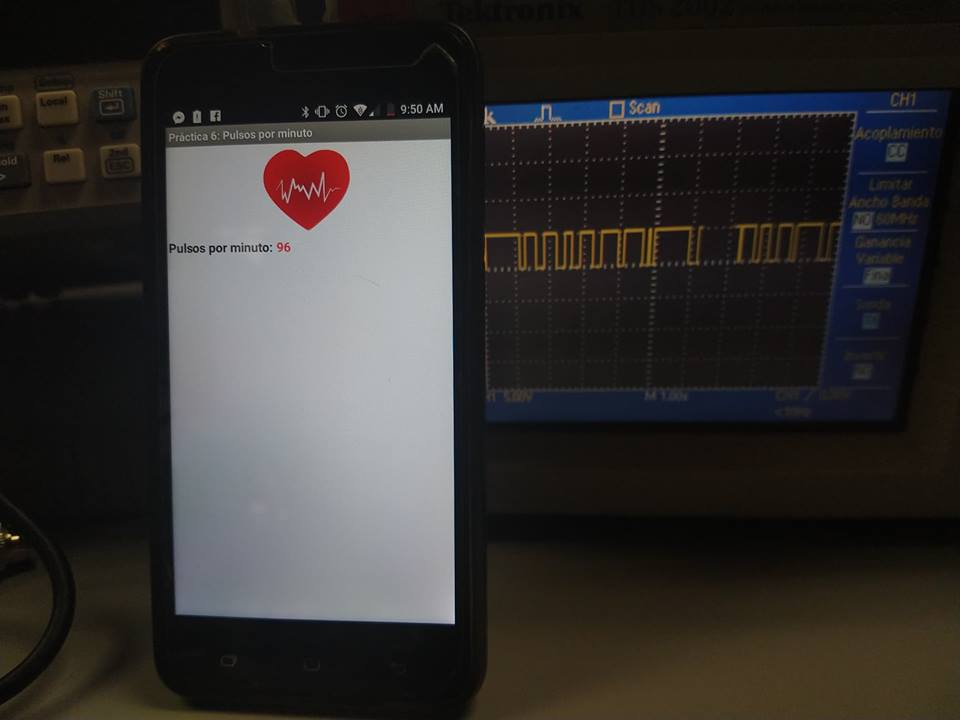
\includegraphics[width=0.8\textwidth]{Practica6/Photos/3.jpg}
             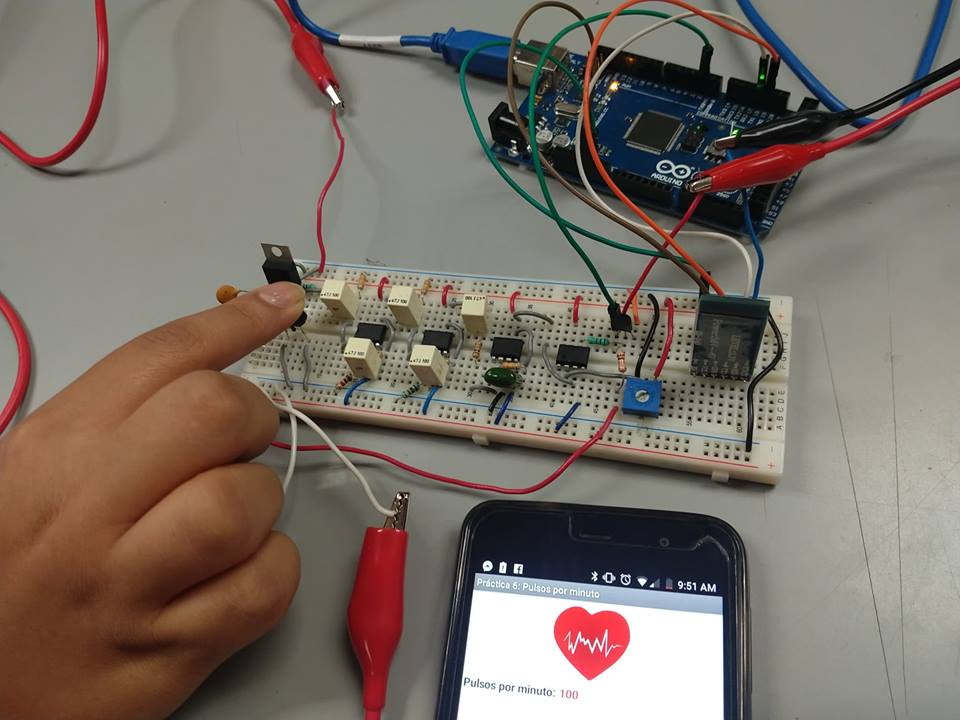
\includegraphics[width=0.8\textwidth]{Practica6/Photos/4.jpg}
    \end{figure}
    \newpage
    \begin{figure}[h!]
                \centering
             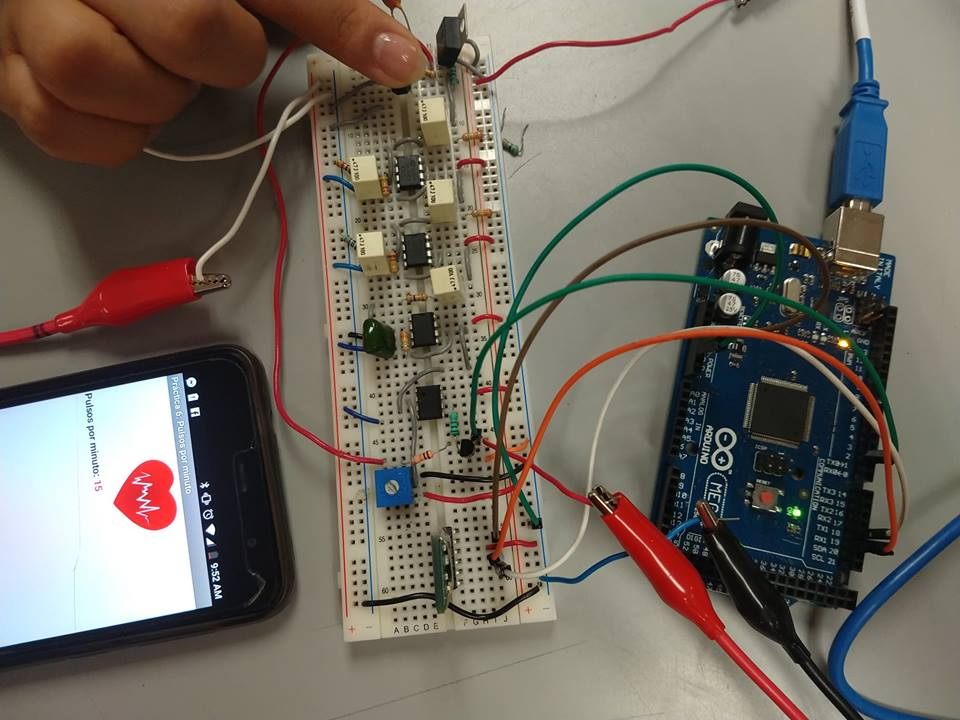
\includegraphics[width=0.8\textwidth]{Practica6/Photos/6.jpg}
             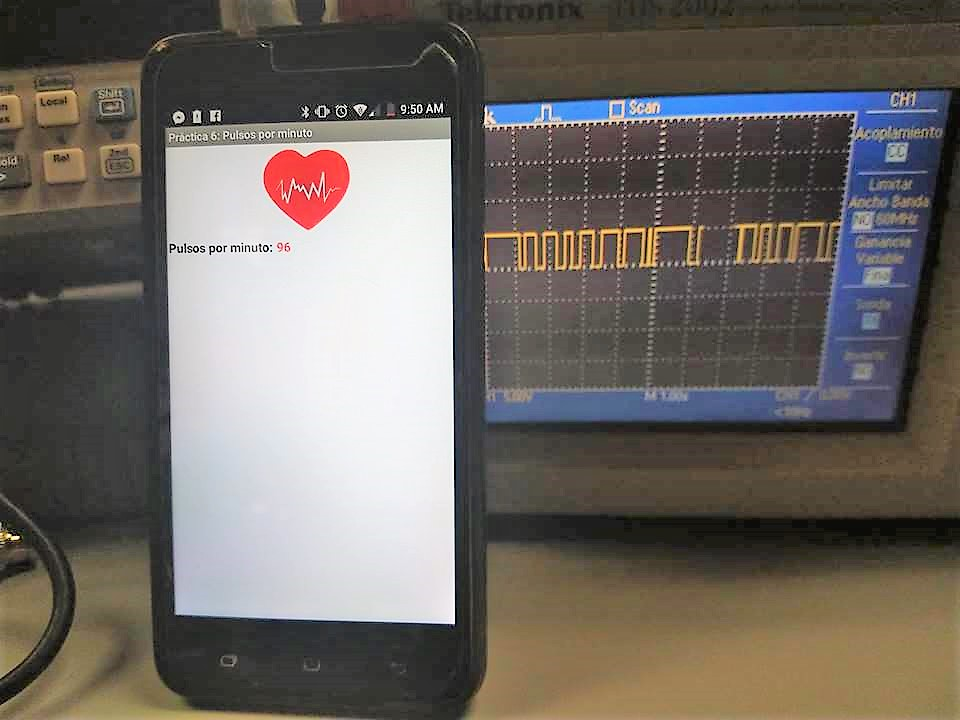
\includegraphics[width=0.8\textwidth]{Practica6/Photos/7.jpg}
    \end{figure}
    
    \newpage
    \section{Observaciones}
    \begin{itemize}
    
    \item[\checkmark] En los 3 vídeos anexados a este reporte se puede visualizar a mayor detalle el \\ comportamiento y funcionamiento del circuito. Link: \textcolor{blue}{\url{https://drive.google.com/drive/folders/1JuevvKissNiwqsKaR3CjCS-S7fGidH1D?usp=sharing}}
    
    \item[\checkmark] También anexamos los códigos tanto del programa de Arduino como de la aplicación desarrollada en MIT App Inventor y su APK. Link: \textcolor{blue}{\url{https://drive.google.com/drive/folders/1RQ2Xoht1R3sdPO-IiZWNO9LnZcn1Rg9G?usp=sharing}}
    
    \item[\checkmark] A veces los valores de pulsaciones por segundo están por debajo de los 50 pulsos o encima de los 100, esto es debido a una mala colocación del dedo en el sensor TCRT5000L, provocando que entre ruido indeseado en la señal, debido a los cambios de luz y sombras, y el Arduino los detecte como pulsos. Basta con colocar el dedo firmemente y relajarlo en el sensor, sin presionar mucho pero también evitando levantarlo.
    \item[\checkmark] Al momento de cargar el programa de Arduino a la placa, es preferible que ningún cable o pines estén conectados al circuito o al HC05, sino hasta que finalice la carga.
    \end{itemize}
    
    %/////////////////////////////////////////////////////////////////
    %                       CONCLUSION
    %/////////////////////////////////////////////////////////////////

    \subsection{ Aguilar Herrera Arianna Itzamina}
        Esta práctica fue, realmente, muy corta, ya que se tomó el funcionamiento de la práctica anterior (práctica 5) y se combinó con el módulo de Bluetooth, para poder mandar la frecuencia cardíaca obtenida mediante el fotopletismógrafo, y enviarla a una aplicación a, en este caso, un teléfono celular, por lo que, podemos concluir que el uso del módulo Bluetooth es muy útil para darle una mejor aplicación a nuestros instrumentos, ya que, mediante Arduino (en este caso se usó Arduino, pero hay otros lenguajes con los que podría funcionar, aunque Arduino es recomendable por su similitud con C) y Bluetooth podemos enviar nuestra variable medida y manipularla a nuestra conveniencia.
    
    \subsection{Ramos Diaz Enrique}
        El principal reto de ésta práctica no fue el armado o acondicionamiento del sensor y la variable que queríamos medir, pues eso se realizo en la práctica anterior, sino la correcta interpretación de ésta, así como la comunicación entre Arduino y una aplicación móvil Android por medio de Bluetooth.
    
        Al principio se intento, por medio de Arduino, leer la cantidad de ceros lógicos (que corresponden a cuando se detecta un pulso) en un periodo de diez segundos y luego multiplicarlo por seis para obtener los pulsos por minuto, pero no tomamos en cuenta lo que realmente importaban era la duración del periodo completo los flancos de subida de la señal cuadrada. Utilizando interrupciones en Arduino, logramos calcular la frecuencia de cada pulso en un minuto.
    
        El siguiente reto era desarrollar la aplicación móvil en donde desplegaremos los resultados. Con ayuda de la página web MIT App Inventor, logramos realizarla de forma muy fácil.
    
        Finalmente quedaba conectar todo y sincronizar el dispositivo móvil con el módulo Bluetooth HC-05, para desplegar los pulsos por minuto que entregaba el fotopletismografo, interpretados y enviados por el Arduino.    
   
   \subsection{Nicolas Sayago Abigail}
        Debido a que el circuito que construimos en la práctica anterior se utilizo, esta práctica fue más sencilla, el problema aquí fue comunicar la señal que nos generaba el sensor con la computadora.
        
        En Arduino existen dos formas de comunicar dependiendo la señal, ya sea analógica o digital, primero nos equivocamos e inicialmente lo hicimos con señal analógica pero a parte de que lleva más lineas de código, si no es conectado correctamente puede causar fallas, corregimos y usamos el código para la señal digital y así fue más fácil y correcto.
        
        La implementación del código paso por varias partes, primero lo intentamos con el delay de Arduino, pero se mejoro con Interrupciones.


    %/////////////////////////////////////////////////////////////////
    %                           ANEXOS
    %/////////////////////////////////////////////////////////////////

    \section{Anexos}
    \subsection{BC547}
    
    Es un transistor amplificador de audio y VHF Freq. Driver con una corriente máxima de colector de 0.6 A, en su composición posee una placa de semiconductor con tres regiones consecutivas de diferente conductibilidad eléctrica los cuales forman dos uniones NPN, las dos regiones extremas tienen un mismo tipo de conductibilidad, la intermedia, conductibilidad de otro tipo, estas son llamadas emisor, colector y base.
    
    \begin{figure}[h!]
                \centering
                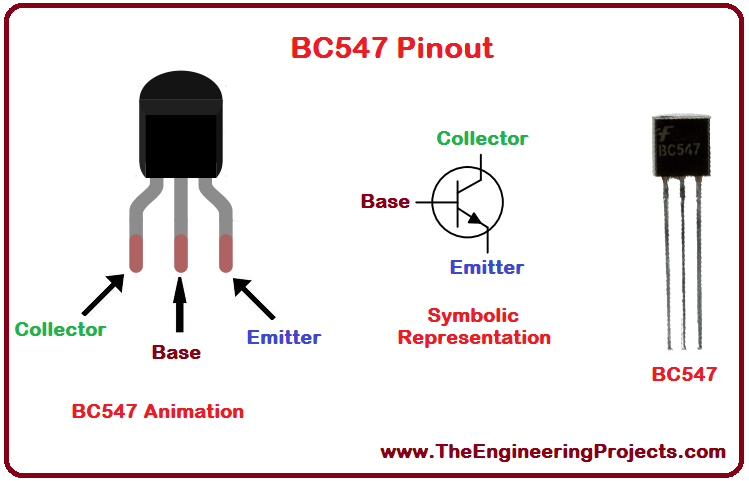
\includegraphics[width=0.55\textwidth]{Practica6/Images/BC547.png}
            \end{figure} 
    \newpage
    \subsection{LM741}
	        \begin{figure}[h!]
                \centering
                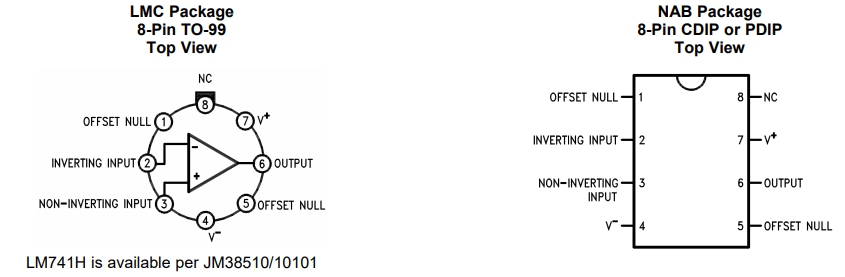
\includegraphics[width=\textwidth]{Practica4/Images/lm741.PNG}
            \end{figure} 
	        El amplificador operacional LM741 debe estar alimentados por una fuente de +12 V y -12 V en serie. [Consultar hoja de especificaciones del LM741].
	        
	        \begin{figure}[h!]
                \centering
                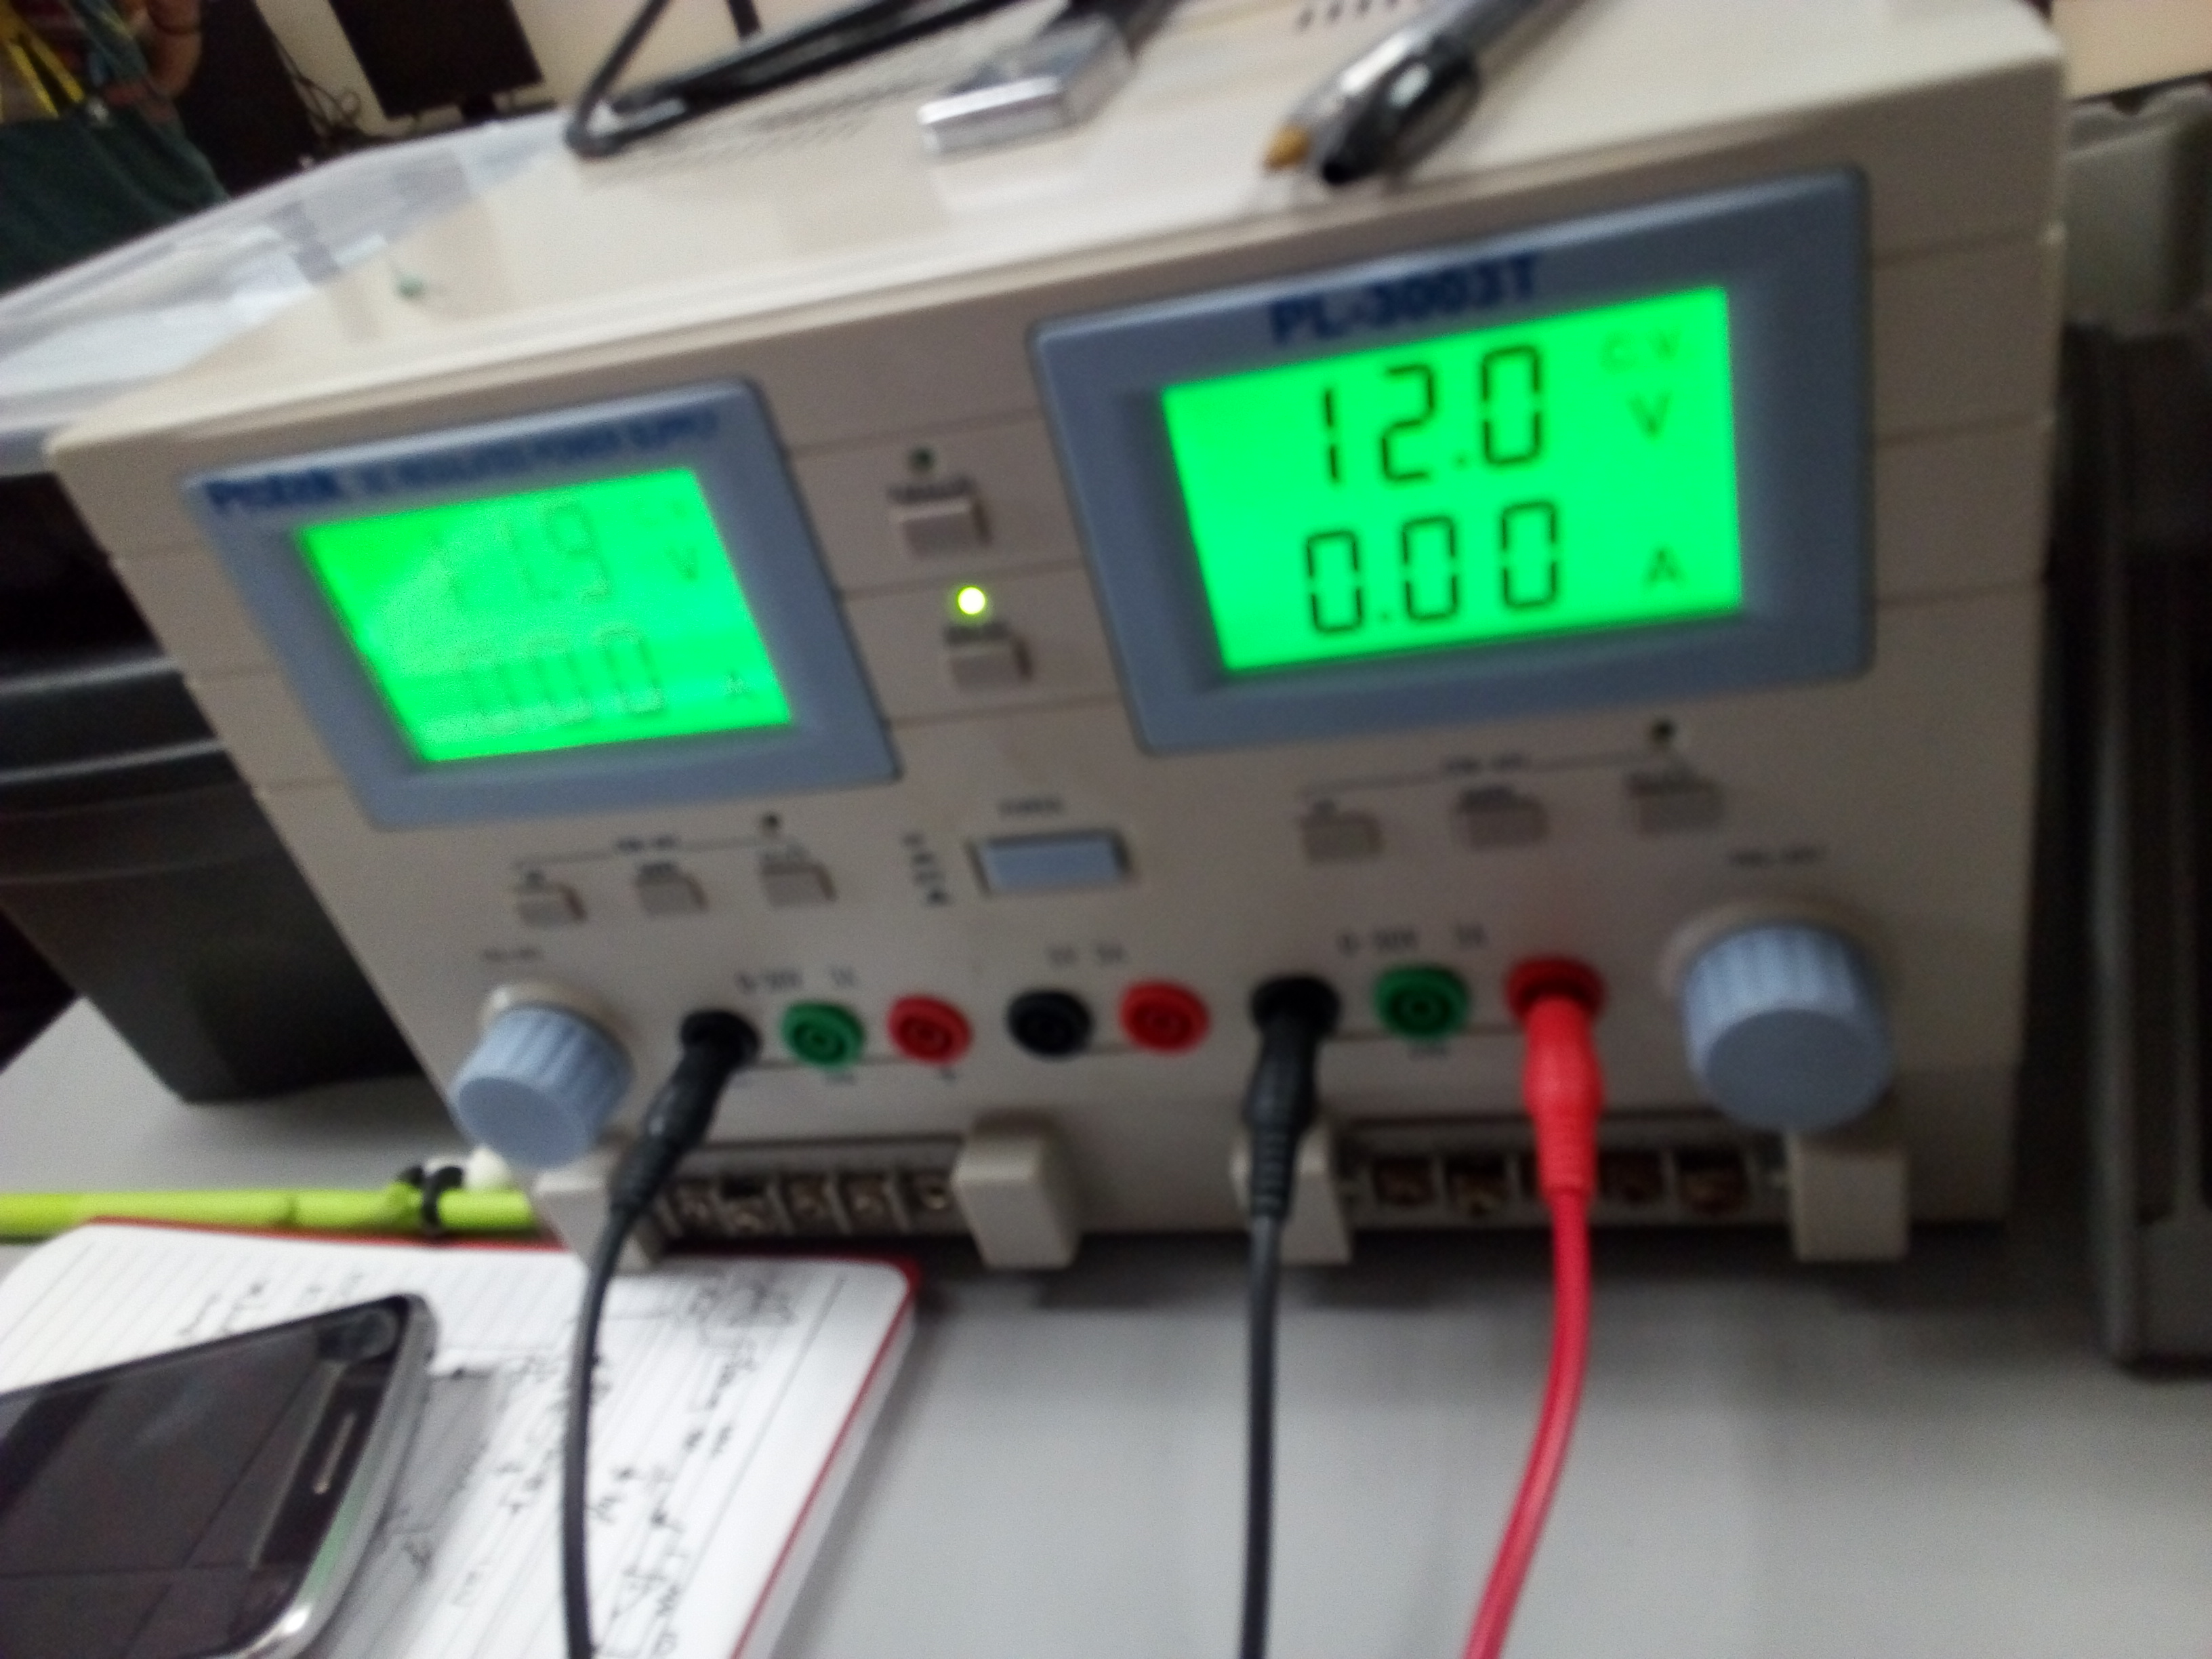
\includegraphics[width=0.7\textwidth]{Sismografo/Images/fuente.jpg}
            \end{figure} 
        \newpage
    \subsection{Arduino Mega}
        \begin{figure}[h!]
                \centering
                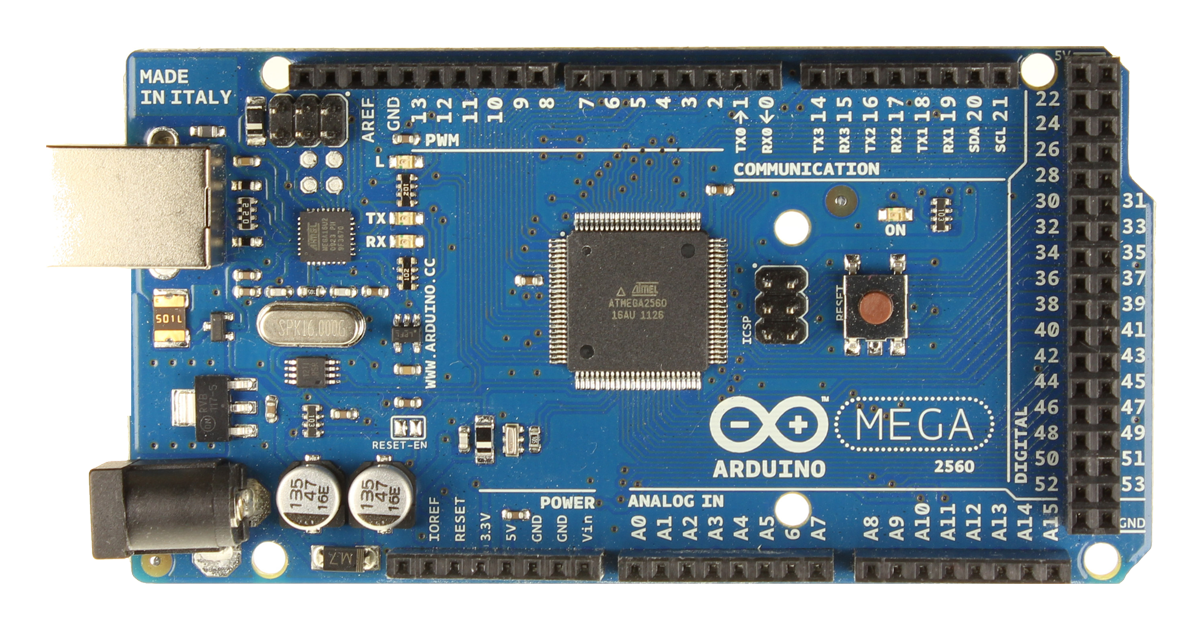
\includegraphics[width=0.8\textwidth]{Practica6/Images/mega.jpg}
            \end{figure} 
    
    \subsection{HC-05}
        \begin{figure}[h!]
                \centering
                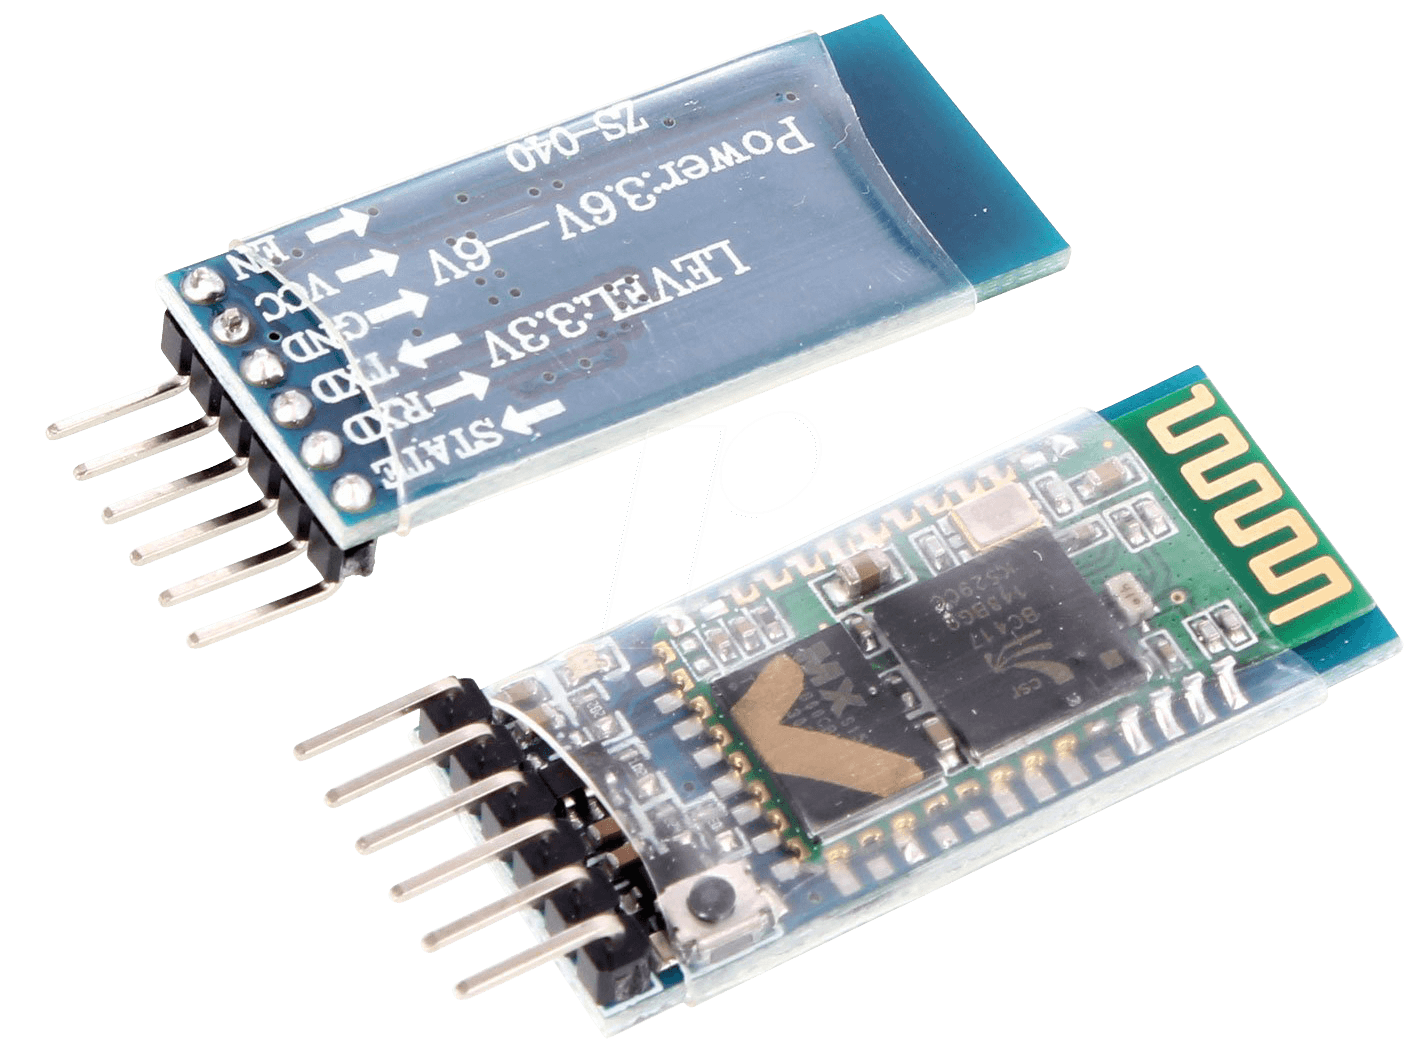
\includegraphics[width=0.8\textwidth]{Practica6/Images/hc05.png}
            \end{figure} 
            
    
    \subsection{Sensor TCRT5000L}

    
    El TCRT5000 y TCRT5000L son sensores reflectivos que incluyen un emisor de infrarrojos y un fototransistor en un paquete de plomo que bloquea la luz visible. El paquete incluye dos clips de montaje. TCRT5000L es la versión de plomo más larga. Debe alimentarse con 5 V.
    
    \begin{figure}[h!]
                \centering
                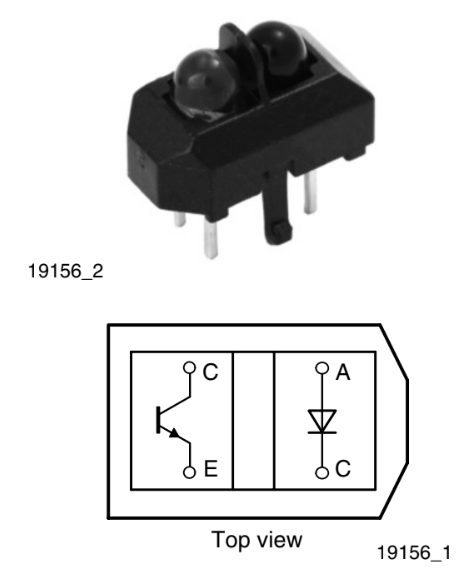
\includegraphics[width=0.5\textwidth]{Practica5/Images/tcrt.PNG}
            \end{figure} 
            
    \subsection{Página Web: MIT App Inventor}
        \begin{figure}[h!]
                \centering
                
\includegraphics[width=0.8\textwidth]{Practica6/Images/mitapp.png}
            \end{figure} 
            
        Para registrarnos y comenzar a crear aplicaciones, únicamente necesitamos una cuenta de Google.
        
        Link: \textcolor{blue}{\url{http://ai2.appinventor.mit.edu/}}
        
    \subsection{Arduino IDE}
        \begin{figure}[h!]
                \centering
                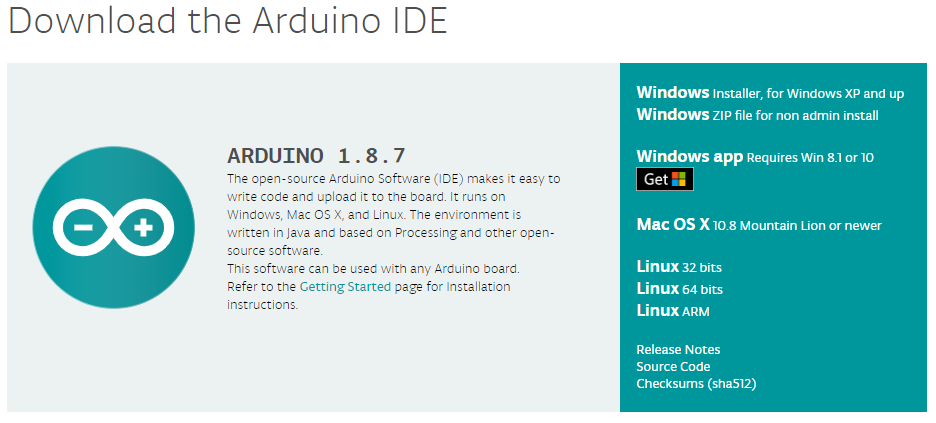
\includegraphics[width=0.9\textwidth]{Practica6/Images/ide.PNG}
            \end{figure} 
            
        
        Link de descarga: \textcolor{blue}{\url{https://www.arduino.cc/en/Main/Software}}
    
       

    %/////////////////////////////////////////////////////////////////
    %                           REFERENCIAS
    %/////////////////////////////////////////////////////////////////

    \nocite{ref1, ref2, ref3, ref4, ref5}
    \bibliography{ref6}
        

    \end{document}
